% ----------------------------------------------------------------
% Chapter 1: Uvod
% ----------------------------------------------------------------
\chapter{Uvod}

Digitalni sadržaj potreban za rad i učenje rijetko se nalazi na jednom mjestu. Dio je u dokumentima, dio na mrežnim stranicama, dio u videozapisima, a dio u uslugama koje se svakodnevno mijenjaju. Korisnik zato često najprije mora pogoditi gdje se informacija nalazi, a tek zatim tražiti pravi izraz unutar tog izvora.

Veliki jezični modeli mijenjaju način postavljanja pitanja jer korisnik više ne mora oblikovati upit kao niz ključnih riječi. Ipak, model sam po sebi ne zna sadržaj privatnih dokumenata niti može pouzdano pratiti izvore koji se stalno mijenjaju. Za takav je slučaj potreban postupak koji prije generiranja odgovora pronalazi relevantan sadržaj i predaje ga modelu. Dohvat potpomognut generiranjem povezuje generativni model s dohvaćenim vanjskim sadržajem te omogućuje da se odgovor oblikuje na temelju pronađenih dokumenata \cite{awsRagGuide}.

Problem koji se razmatra u ovom radu zato nije samo spremanje izvora na jedno mjesto. Potrebno ih je pretvoriti u oblik pogodan za pretraživanje, povezati ih s razgovorom i pritom sačuvati vezu između odgovora i izvornog sadržaja. Ta je veza važna jer korisnik mora moći otvoriti citat, pročitati ulomak i provjeriti kontekst iz kojeg je odgovor izveden. Sustav uz to mora obrađivati veći broj izvora bez blokiranja sučelja, odvojiti podatke različitih prostora znanja i podržati suradnju korisnika s različitim ovlastima.

Cilj rada je oblikovati i razviti mrežnu aplikaciju za izgradnju, organizaciju i korištenje baza znanja uz primjenu dohvata potpomognutog generiranjem. Korisnik u aplikaciji stvara prostor znanja, dodaje datoteke, mrežne stranice i videozapise te povezuje podržane vanjske izvore podataka. Nakon indeksiranja može postavljati pitanja prirodnim jezikom, primati odgovor u stvarnom vremenu i pregledati izvore na kojima se odgovor temelji. Isti se tijek može koristiti za pretraživanje projektne dokumentacije, pripremu sažetaka i analiza, istraživanje sadržaja iz više izvora te dijeljenje uređenog znanja unutar tima.

Razvijeno rješenje ima četiri glavna dijela: klijentsku aplikaciju, poslužiteljsku aplikaciju, relacijsku bazu podataka s vektorskom pohranom i pozadinsku obradu dugotrajnih zadataka. Izvori se najprije pretvaraju u standardizirane dokumente. Zatim se dijele na manje cjeline i indeksiraju za kombinirano semantičko i tekstualno pretraživanje. Dohvaćeni se sadržaj ponovno rangira i prosljeđuje jezičnom modelu, a odgovor se korisniku vraća zajedno s citatima. Stanje obrade dokumenata i povezanih izvora prenosi se korisničkom sučelju događajima poslužitelja, pa korisnik može pratiti zadatke bez ručnog osvježavanja stranice.

Funkcionalnosti su podijeljene prema razini pristupa. Neregistrirani korisnik može pristupiti prijavi, registraciji i javno objavljenom sadržaju. Član prostora znanja radi s dokumentima, razgovorima, bilježnicama, poveznicima i konfiguracijama modela, ali samo u okviru svoje uloge. Vlasnik, urednik i pregledavatelj zato nemaju iste radnje nad zajedničkim sadržajem. Odvojeno od tog tijeka, administratorski dio sustava prati korisnike, pakete, potrošnju kredita, naplatu i stanje platforme.

Glavni doprinos rada jest povezivanje tih dijelova u jedan tijek upravljanja znanjem. Razvijen je postupak unosa heterogenih izvora, njihove asinkrone obrade i pohrane u obliku pogodnom za hibridno pretraživanje. Razvijeno je razgovorno sučelje koje podržava strujanje odgovora, citiranje izvora, analizu slika i dodavanje novih izvora iz samog razgovora. Podaci su organizirani prema prostorima znanja, uz upravljanje članovima i ovlastima, periodičko indeksiranje povezanih usluga te dnevničke zapise za praćenje obrade.

Rad je usmjeren na oblikovanje i implementaciju aplikacijskog sustava. Ne obuhvaća razvoj ni uvježbavanje novog velikog jezičnog modela. Umjesto toga, aplikacija koristi postojeće jezične modele za pretraživanje i obradu korisničkih izvora znanja. Naglasak rada je na povezivanju tih modela s postupcima unosa, indeksiranja, pretraživanja i prikaza izvora te na provjeri razvijenih funkcionalnosti kroz odabrane scenarije ispitivanja.

Drugo poglavlje uvodi samo pojmove potrebne za razumijevanje rada sustava: agentske sustave, dohvat potpomognut generiranjem, vektorske baze podataka te semantičko i hibridno pretraživanje. Treće poglavlje zatim prelazi s podloge na razvijeno rješenje. Najprije opisuje arhitekturu i model podataka, a potom korisničke tijekove za neregistrirane korisnike, članove prostora znanja i administratore. Četvrto poglavlje sažima ostvarene doprinose, ograničenja i mogućnosti daljnjeg razvoja.

% ----------------------------------------------------------------
% Chapter 2: Teorijska podloga
% ----------------------------------------------------------------
\chapter{Teorijska podloga}

Razvijeni sustav može se razumjeti kroz put koji prolazi jedno korisničko pitanje. Najprije treba odlučiti koje radnje sustav smije poduzeti, zatim treba pronaći relevantne dijelove izvora, a na kraju model mora iz tog konteksta oblikovati odgovor. Zbog toga su u ovom poglavlju objašnjeni samo pojmovi koji sudjeluju u tom putu: agentski sustavi, dohvat potpomognut generiranjem, vektorske baze podataka te semantičko i hibridno pretraživanje. Poglavlje ne opisuje velike jezične modele općenito, nego mehanizme koji su potrebni za razumijevanje razvijene aplikacije.

\section{Agentski sustavi}

U uobičajenom programskom postupku redoslijed operacija unaprijed je zadan. Isti ulaz prolazi kroz iste korake, a odluke su zapisane pravilima u programskom kôdu. Agentski sustav razlikuje se po tome što na temelju cilja i trenutačnog stanja odabire sljedeću radnju. Veliki jezični model pritom nije cijeli agent, nego dio sustava koji tumači zahtjev, procjenjuje dostupne mogućnosti i odlučuje treba li odgovoriti ili upotrijebiti neki alat. Alati mogu obuhvaćati pretraživanje baze znanja, dohvat mrežnog sadržaja, obradu datoteke ili pozivanje druge vanjske usluge.

Takav se rad može prikazati kao ponavljajući ciklus. Dokumentacija razvojnog okruženja Visual Studio Code opisuje agentsku petlju u kojoj agent u svakom koraku procjenjuje napredak, odabire sljedeću radnju i rezultat te radnje koristi kao ulaz za novu odluku \cite{vscodeAgents}. Slika~\ref{fig:agentski-ciklus} prikazuje taj tijek. Agent najprije prima korisnički cilj. Ako raspoloživi kontekst nije dovoljan za odgovor, bira alat i oblikuje njegove ulazne podatke. Rezultat alata postaje novo opažanje na temelju kojeg agent ponovno odlučuje. Ciklus završava kada je cilj ostvaren, kada više nije moguće napraviti koristan korak ili kada je dosegnuto zadano ograničenje izvođenja.

\begin{figure}[H]
    \centering
    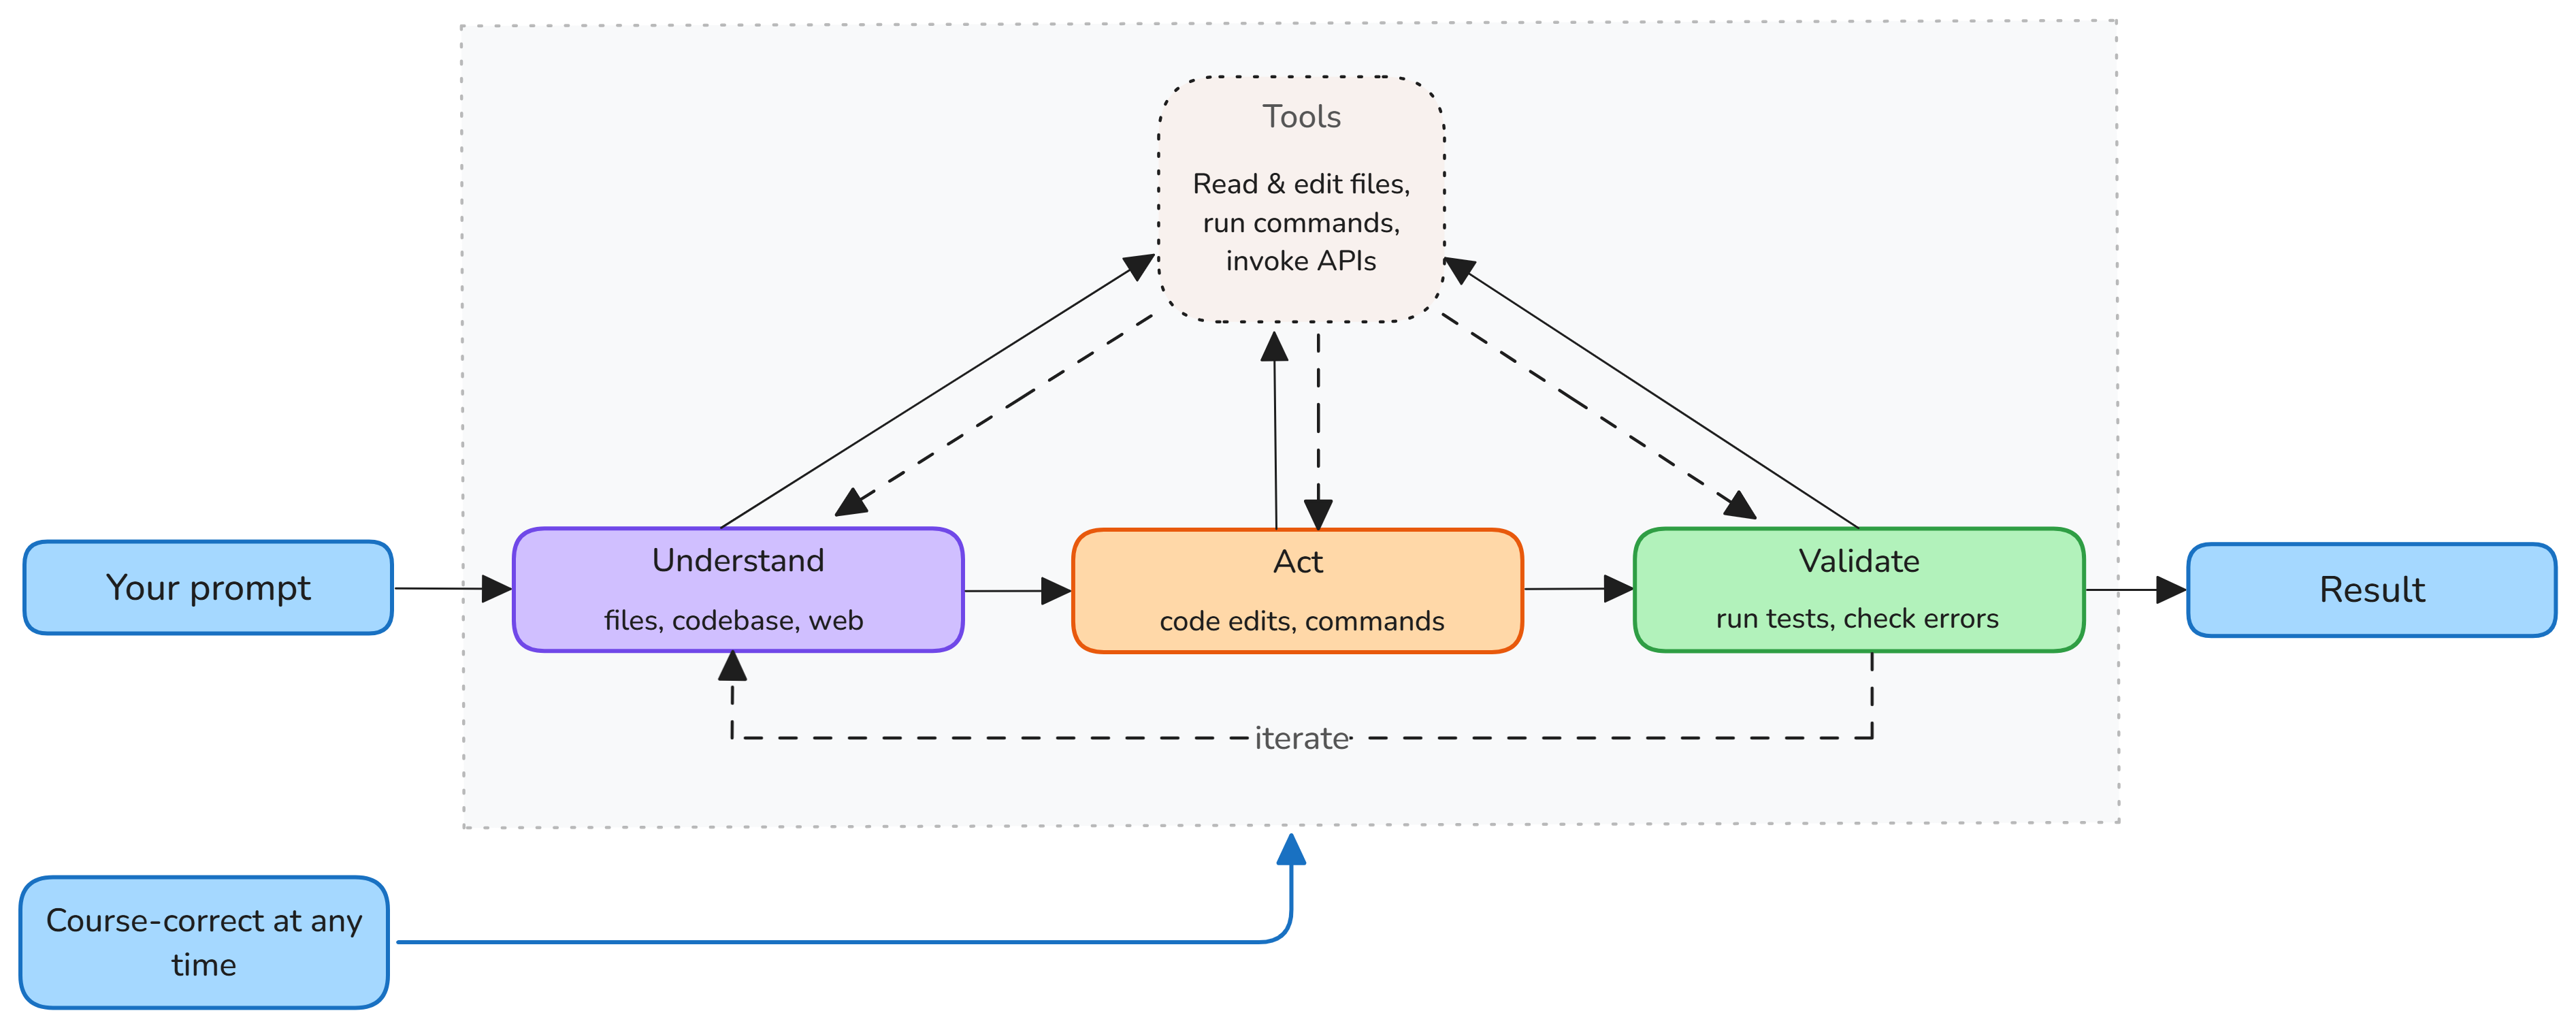
\includegraphics[width=\textwidth]{assets/source_agent_loop.png}
    \DiffComment{Ispod slika nije potrebno pisati riječ Izvor. Npr.\newline Osnovni tijek odgovaranja u sustavu RAG. Izvor: [1]\newline napravite ovako> Osnovni tijek odgovaranja u sustavu RAG [1]}
    \caption{Ciklus razumijevanja, djelovanja i provjere agentskog sustava\DiffReplaceInline{. Izvor:}{~}\cite{vscodeAgents}}
    \label{fig:agentski-ciklus}
\end{figure}

\DiffComment{Na stranici 5 se spominje LangChain koji pada s neba. Stavite riječ prije, npr. Alat LangChain, razvojni okvir LangChain, odnosno objasnite što je to prije spominjanja.}
\DiffComment{Ispis 1 - nije jasno je li ovo vaš kôd ili nekog općenitog modela/agenta. U poglavlju govorite o teoretskoj podlozi, a stavljate kod što je zbunjujuće. Ako je kod vaš, naglasite to i ubacite par rečenica uvoda/pojašnjenja. Zapravo fraza "u razvijenom sustavu" je nejasna. Jel se referirate na svoj rad? Napišite to jasnije.}
\DiffReplace{LangChain opisuje agent kao model koji poziva dostupne alate u petlji sve dok ne oblikuje završni odgovor ili ne dosegne ograničenje izvođenja \cite{langchainAgents}.

U razvijenom sustavu alati se grade iz ovisnosti dostupnih prijavljenom korisniku, a zatim se zajedno s odabranim modelom, sistemskom uputom i spremnikom stanja predaju funkciji \texttt{createDeepAgent}. Sažeti dio tog postupka prikazan je u ispisu~\ref{code:stvaranje-agenta}.}{U implementaciji je upotrijebljen razvojni okvir LangChain, skup biblioteka za povezivanje jezičnih modela, alata i tijeka njihove obrade. U kontekstu agenata LangChain opisuje agenta kao model koji poziva dostupne alate u petlji sve dok ne oblikuje završni odgovor ili ne dosegne ograničenje izvođenja \cite{langchainAgents}.

U aplikacijskom sustavu razvijenom u ovom diplomskom radu alati se grade iz ovisnosti dostupnih prijavljenom korisniku. Zatim se zajedno s odabranim modelom, sistemskom uputom i spremnikom stanja predaju funkciji \texttt{createDeepAgent}. Ispis~\ref{code:stvaranje-agenta} prikazuje skraćeni isječak vlastitog programskog kôda iz servisne klase za agentski razgovor. Isječak izdvaja samo sastavljanje agenta: iz pripremljenih ovisnosti stvara skup alata, oblikuje sistemsku uputu i povezuje ih s odabranim jezičnim modelom.}

\noindent\begin{minipage}{\textwidth}
\begin{lstlisting}[
    caption={Stvaranje agenta s modelom i alatima u razvijenom sustavu},
    label={code:stvaranje-agenta}
]
const tools = buildTools(dependencies);
const systemPrompt = buildSystemPrompt(language);

return createDeepAgent({
  model: llm,
  tools,
  systemPrompt,
  checkpointer,
});
\end{lstlisting}
\end{minipage}

Iz toga proizlazi važno ograničenje: ponašanje agenta ne određuje samo tekst upute jezičnom modelu. Na njega utječu skup dostupnih alata, opis svakog alata, sadržaj razgovora, rezultati prethodnih radnji i pravila za prekid izvođenja. Alat mora imati jasnu svrhu i ulazne podatke jer agent iz tog opisa odlučuje kada će ga upotrijebiti. Rezultat alata mora biti predvidljiv kako bi se mogao uključiti u sljedeći korak. Sloboda odlučivanja time ostaje vezana uz radnje koje aplikacija izričito dopušta.

Agentski pristup koristan je kada zahtjev nije moguće pouzdano riješiti jednom unaprijed određenom operacijom. Pitanje može zahtijevati više pretraživanja, promjenu upita nakon nepotpunog rezultata ili spajanje podataka iz različitih izvora. Cijena takve fleksibilnosti je dulje izvođenje i veća mogućnost pogrešne odluke. Zbog toga sustav treba bilježiti provedene radnje, ograničiti njihov broj i provjeravati ovlasti prije pristupa podacima. U razvijenoj aplikaciji najvažniji alat agenta jest pretraživanje odabranog prostora znanja. Sljedeći odjeljak objašnjava kako se pronađeni sadržaj pretvara u podlogu za odgovor.

\section{Sustavi za dohvat potpomognut generiranjem}

Dohvat potpomognut generiranjem (engl. \textit{retrieval-augmented generation}, RAG) povezuje generativni jezični model s vanjskom zbirkom podataka. Umjesto da se odgovor temelji samo na znanju sadržanom u parametrima modela, prije generiranja pronalaze se dijelovi izvora povezani s korisničkim pitanjem. Ti se dijelovi pridružuju pitanju kao kontekst iz kojeg model oblikuje odgovor. Tehnički vodič AWS-a opisuje RAG kao postupak u kojem se vanjski podaci dohvaćaju iz vektorske baze i dodaju upitu prije njegova slanja jezičnom modelu \cite{awsRagGuide}.

Rad sustava RAG ima dva povezana toka, prikazana na slici~\ref{fig:rag-tijek}. Prvi tok događa se prije pitanja korisnika. Dokumenti se dohvaćaju iz podržanih izvora, tekst se čisti i dijeli na manje cjeline, a svaka se cjelina zajedno s metapodacima priprema za pretraživanje. Podjela je potrebna jer cijeli dokument često sadrži više tema, dok je za odgovor relevantan samo njegov manji dio. Premale cjeline mogu izgubiti potreban kontekst, a prevelike mogu unijeti mnogo nepovezanog sadržaja. Veličina i način preklapanja dijelova zato utječu na kvalitetu kasnijeg dohvata.

Drugi tok započinje korisničkim pitanjem. Sustav pretražuje pripremljeni indeks, odabire najbolje rangirane cjeline i zajedno s pitanjem prosljeđuje ih jezičnom modelu. Model tada ne pretražuje bazu samostalno, nego sastavlja odgovor iz konteksta koji mu je dostavljen. Uz svaki dohvaćeni dio potrebno je sačuvati podatke o izvornom dokumentu kako bi odgovor mogao sadržavati poveznice ili citate. Korisnik tako može otvoriti izvor i provjeriti je li odgovor vjerodostojno prenio pronađeni sadržaj.

\begin{figure}[H]
    \centering
    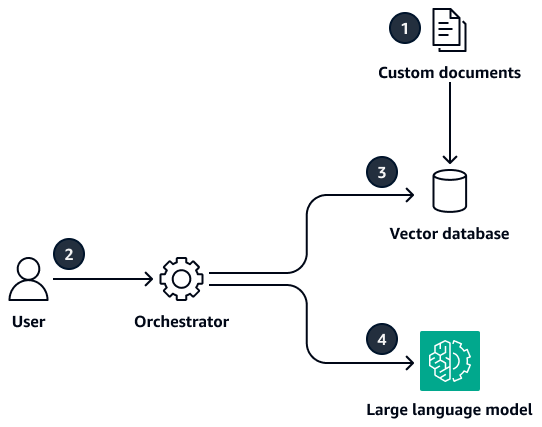
\includegraphics[width=0.68\textwidth]{assets/source_rag_overview.png}
    \DiffComment{Ispod slika nije potrebno pisati riječ Izvor. Npr.\newline Osnovni tijek odgovaranja u sustavu RAG. Izvor: [1]\newline napravite ovako> Osnovni tijek odgovaranja u sustavu RAG [1]}
    \caption{Osnovni tijek odgovaranja u sustavu RAG\DiffReplaceInline{. Izvor:}{~}\cite{awsRagGuide}}
    \label{fig:rag-tijek}
\end{figure}

RAG ne jamči točan odgovor samim time što je uz model povezan indeks. Kvaliteta rezultata ovisi o cijelom lancu. Tekst mora biti pravilno izdvojen, relevantna cjelina mora biti pronađena, njezin sadržaj mora stati u raspoloživi kontekst, a model mora odgovor oblikovati prema tom sadržaju. Ako dohvat izostavi ključan dio dokumenta, model ga u fazi generiranja ne može pouzdano nadoknaditi. Pronađeni tekst usto može biti zastario, proturječan ili nedovoljno precizan. Citiranje zato nije samo oznaka podrijetla podataka. Ono korisniku daje mjesto na kojem može provjeriti je li izvor primjeren pitanju.

Odvajanje zbirke dokumenata od parametara modela ima praktičnu prednost: sadržaj se može dodavati, uklanjati i ponovno indeksirati bez uvježbavanja novog modela. Ista se generativna komponenta može povezati s različitim prostorima znanja, dok se pristup ograničava na izvore dopuštene pojedinom korisniku. Da bi takav dohvat prepoznao i sadržaj koji ne ponavlja iste riječi kao pitanje, tekst se prikazuje vektorima i pohranjuje u sustav prilagođen usporedbi tih prikaza.

\section{Vektorske baze podataka}

Semantički dohvat temelji se na ugradnjama (engl. \textit{embeddings}), brojčanim prikazima teksta u obliku vektora. Model za izradu ugradnji preslikava pitanje i dijelove dokumenata u isti višedimenzijski prostor. Vektori tekstova sličnog značenja trebali bi u tom prostoru biti bliži od vektora sadržajno nepovezanih tekstova. Zbog toga je moguće pronaći odlomak povezan s pitanjem čak i kada pitanje i odlomak ne koriste potpuno jednake riječi. Google Cloud u vodiču o vektorskim bazama opisuje ugradnje kao brojčane prikaze nestrukturiranih podataka kod kojih blizina u vektorskom prostoru predstavlja semantičku povezanost \cite{googleVectorDatabase}.

Vektorska baza podataka pohranjuje takve vektore zajedno s pripadajućim sadržajem i omogućuje pretraživanje najbližih susjeda. Za upit se najprije izračuna vektor, nakon čega se njegova udaljenost uspoređuje s vektorima u zbirci. Često se koristi kosinusna udaljenost, koja uspoređuje smjer vektora, dok druga rješenja mogu primjenjivati euklidsku udaljenost ili skalarni produkt. Rezultat nije odgovor, nego poredak zapisa prema odabranoj mjeri sličnosti. Tekst i metapodaci pronađenih zapisa zatim se vraćaju postupku RAG.

Slika~\ref{fig:vektorska-baza} prikazuje vezu između izvornog sadržaja, modela za izradu ugradnji i vektorske baze. Isti model pretvara dokumente i korisnički upit u kompatibilne vektore. Baza pronalazi pohranjene vektore najbliže vektoru upita i preko njih vraća povezani izvorni sadržaj.

\begin{figure}[H]
    \centering
    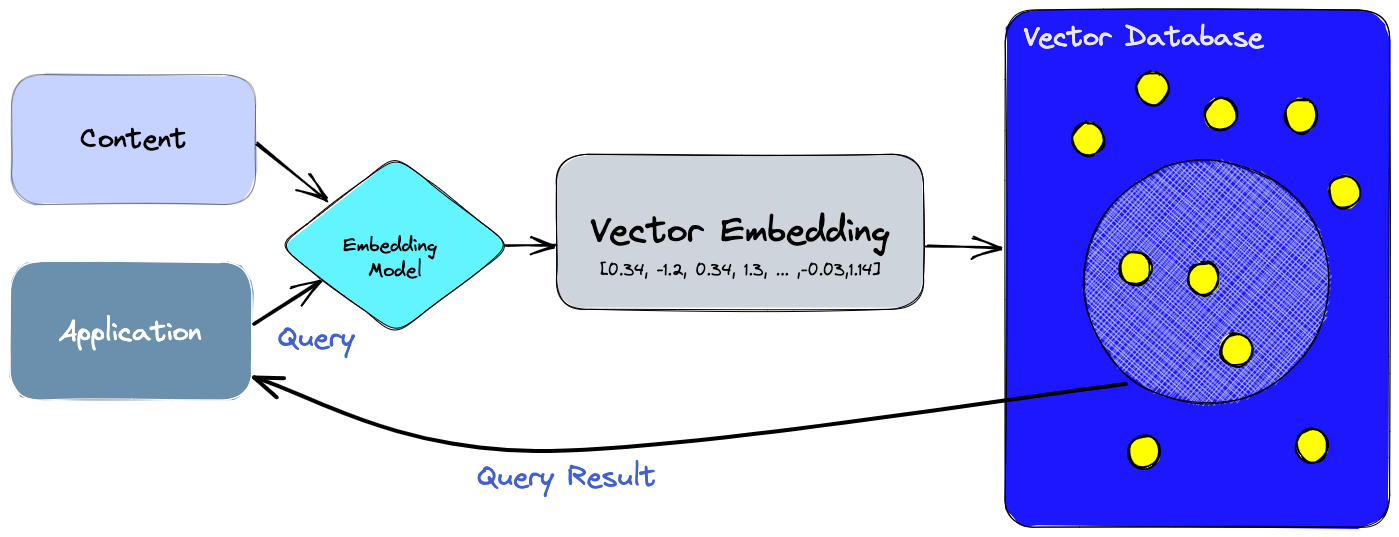
\includegraphics[width=\textwidth]{assets/source_vector_database.png}
    \DiffComment{Ispod slika nije potrebno pisati riječ Izvor. Npr.\newline Osnovni tijek odgovaranja u sustavu RAG. Izvor: [1]\newline napravite ovako> Osnovni tijek odgovaranja u sustavu RAG [1]}
    \caption{Uloga modela za izradu ugradnji i vektorske baze podataka\DiffReplaceInline{. Izvor:}{~}\cite{pineconeVectorDatabase}}
    \label{fig:vektorska-baza}
\end{figure}

Dokumentacija integracije \texttt{OpenAIEmbeddings} razlikuje metodu \texttt{embedDocuments}, koja obrađuje dokumente, od metode \texttt{embedQuery}, koja izrađuje vektor pojedinačnog upita \cite{langchainOpenAIEmbeddings}. OpenAI API vraća ugradnju kao polje decimalnih brojeva čija duljina ovisi o odabranom modelu \cite{openAIEmbeddingsApi}. Ispis~\ref{code:izrada-ugradnje} prikazuje odgovarajući dio razvijenog servisa. Servis preuzima naziv modela iz konfiguracije, stvara objekt \texttt{OpenAIEmbeddings} i za primljeni tekst vraća vektor upita. Taj se vektor koristi u usporedbi s vektorima pohranjenih dijelova dokumenata.

\noindent\begin{minipage}{\textwidth}
\begin{lstlisting}[
    caption={Izrada vektorske ugradnje korisničkog upita},
    label={code:izrada-ugradnje}
]
this.embeddingModel = new OpenAIEmbeddings({
  model: embeddingConfig.model,
});

async embed(text: string): Promise<number[]> {
  return await this.embeddingModel.embedQuery(text);
}
\end{lstlisting}
\end{minipage}

Pojam vektorske baze ne mora označavati zaseban poslužiteljski proizvod. Postojeće baze podataka mogu se proširiti vektorskim tipom i operatorima za udaljenost. Proširenje pgvector za PostgreSQL podržava pohranu vektora, egzaktno i približno pretraživanje najbližih susjeda te više mjera udaljenosti \cite{pgvector}. U razvijenoj aplikaciji vektorska pohrana nalazi se uz relacijske podatke o dokumentima, korisnicima i prostorima znanja. Zbog toga se semantički rezultat može ograničiti metapodacima, primjerice pripadnošću određenom prostoru znanja, prije nego što se sadržaj vrati agentu.

Kod egzaktnog pretraživanja udaljenost se razmatra za sve dopuštene vektore, čime se dobiva točan poredak za zadanu mjeru, ali trošak raste s veličinom zbirke. Približni indeksi smanjuju broj usporedbi i ubrzavaju dohvat, uz mogućnost da neki od stvarno najbližih zapisa ne budu pronađeni. pgvector, primjerice, podržava indekse HNSW i IVFFlat te izričito navodi odnos brzine i odziva prema potpunosti dohvata \cite{pgvector}. Izbor indeksa i njegovih parametara zato nije samo tehničko pitanje performansi; utječe i na sadržaj koji će biti dostupan generativnom modelu.

Vektorska sličnost dobro povezuje parafraze i tematski srodne izraze, ali ne zamjenjuje sve oblike tekstualnog pretraživanja. Oznaka proizvoda, osobno ime, kratica ili točan broj mogu biti važni upravo zbog doslovnog zapisa. Zbog toga se u sustavima RAG semantički rezultat često povezuje s rezultatom pretraživanja riječi i izraza.

\section{Semantičko i hibridno pretraživanje u sustavima RAG}

Semantičko pretraživanje pronalazi sadržaj prema značenju korisničkog pitanja, a ne samo prema podudaranju riječi. Pitanje o dodavanju člana u prostor znanja tako može pronaći tekst koji opisuje pozivanje suradnika, iako nisu upotrijebljene iste riječi. To je važno u sustavima RAG jer korisnik ne mora poznavati točan izraz kojim je tražena informacija zapisana u dokumentu.

\DiffComment{str 9 - riječ "poredava" nije dobra\newline - slaže, sortira...}
Ipak, semantičko pretraživanje nije jednako pouzdano za svaku vrstu upita. Točni nazivi proizvoda, kratice, osobna imena i identifikatori često se bolje pronalaze tekstualnim pretraživanjem. PostgreSQL takvo pretraživanje provodi nad normaliziranim riječima iz dokumenta i korisničkog upita te rezultate \DiffReplaceInline{poredava}{sortira} prema njihovoj podudarnosti \cite{postgresqlTextSearch}. Tekstualno pretraživanje zato dobro pronalazi doslovno navedene pojmove, ali može propustiti sadržaj u kojem je ista namjera izražena drugim riječima.

Hibridno pretraživanje povezuje prednosti obaju pristupa. Semantičko i tekstualno pretraživanje izvode se nad istim skupom dokumenata, a njihovi se rezultati spajaju u zajednički poredak \cite{azureHybridSearch}. Prednost dobivaju cjeline koje su relevantne prema značenju pitanja, prema njegovim ključnim riječima ili prema oba kriterija. Time se smanjuje mogućnost da važan dokument bude izostavljen samo zato što korisnik nije upotrijebio isti izraz kao njegov autor.

\DiffComment{str 26\newline "postupkom recipročnog fuzioniranja rangova" > to je valjda RRF? Nigdje niste to rekli, ovdje ovaj složeni pojam pada s neba. Raspišite uvod u ovu rečenicu.}
\DiffReplace{U razvijenom sustavu oba načina pretraživanja stvaraju vlastiti popis rezultata. Njihovi se položaji zatim objedinjuju postupkom recipročnog fuzioniranja rangova (engl. \textit{reciprocal rank fusion}, RRF). Za razumijevanje aplikacije nije potreban matematički prikaz postupka. Važno je da RRF daje prednost cjelinama koje se dobro pojavljuju u jednom ili u oba poretka. Najbolje rangirane cjeline predaju se agentu kao kontekst za oblikovanje odgovora, a njihovi metapodaci omogućuju prikaz izvora. Time završava put od korisničkog pitanja do sadržaja koji model smije koristiti.}{U razvijenom sustavu semantičko i tekstualno pretraživanje najprije stvaraju dva odvojena poretka istih cjelina. Njihovi se položaji zatim objedinjuju metodom recipročnog fuzioniranja rangova (engl. \textit{reciprocal rank fusion}, RRF). RRF ne uspoređuje izravno početne ocjene dvaju pretraživanja, nego za svaku cjelinu uzima njezin položaj \(r\) na svakom popisu: prva cjelina ima \(r=1\), druga \(r=2\), a njezin doprinos iznosi \(1/(60+r)\). Doprinosi semantičkog i tekstualnog poretka zbrajaju se u konačni rezultat. Cjelina koja je visoko na oba popisa zato dobiva dva velika doprinosa, dok cjelina pronađena samo jednim pristupom dobiva jedan doprinos. Nakon sortiranja prema tom zbroju najbolje rangirane cjeline predaju se agentu kao kontekst za oblikovanje odgovora, a njihovi metapodaci omogućuju prikaz izvora. Time završava put od korisničkog pitanja do sadržaja koji model smije koristiti.}

% ----------------------------------------------------------------
% Chapter 3: Izgled i funkcionalnosti sustava
% ----------------------------------------------------------------
\chapter{Izgled i funkcionalnosti sustava}

\DiffComment{str 11\newline Prostor znanja predstavlja središnju organizacijsku cjelinu razvijenog sustava\newline > Prostor znanja predstavlja središnju organizacijsku cjelinu sustava razvijenog u ovom diplomskom radu. Općenito pojasnite riječ "sustava" gdje god ima smisla, posebno u početnim dijelovima rada - naglasite da je to vaš sustav, vaš rad}
\DiffReplace{Prostor znanja središnja je organizacijska cjelina razvijenog sustava.}{Prostor znanja središnja je organizacijska cjelina aplikacijskog sustava razvijenog u ovom diplomskom radu.} U njemu se nalaze izvori, obrađeni dokumenti, razgovori, bilježnice i članovi s pripadajućim ovlastima. Time se sadržaj ne promatra kao skup nepovezanih datoteka, nego kao radni prostor u kojem isti izvori mogu služiti čitanju, pretraživanju i razgovoru s agentom.

Životni ciklus sadržaja zato ima stalni redoslijed. Izvor se dodaje u prostor, obrađuje u pozadini, priprema za pretraživanje i zatim koristi kao podloga za odgovor. Arhitektura i model podataka oblikovani su tako da taj tijek ostane jednak neovisno o vrsti izvora, dok korisničko sučelje prikazuje samo radnje dopuštene ulozi prijavljenog korisnika.

\section{Struktura sustava}

\DiffReplace{Sustav se sastoji od klijentske aplikacije, poslužiteljske aplikacije, baze podataka i pozadinskih procesa.}{Aplikacijski sustav razvijen u ovom diplomskom radu sastoji se od klijentske aplikacije, poslužiteljske aplikacije, baze podataka i pozadinskih procesa.} Klijentska aplikacija razvijena je u razvojnom okviru Next.js i izvodi se u pregledniku. Ona šalje zahtjeve HTTP poslužiteljskoj aplikaciji i prikazuje promjene stanja, ali nema izravan pristup bazi podataka. Poslužiteljska aplikacija razvijena je u okviru NestJS. Njezini su moduli podijeljeni prema poslovnim cjelinama: autentikaciji, prostorima znanja, dokumentima, razgovorima, bilježnicama, poveznicima, konfiguracijama modela, pretplatama i administraciji.

\DiffComment{str 48\newline "Bullov red" > što je to? Ne možete složene pojmove kao ovaj koristiti tako da padnu s neba}
\DiffReplace{Međusobni odnos glavnih komponenti prikazan je na slici~\ref{fig:arhitektura-sustava}. Kraće operacije obrađuju se unutar jednog zahtjeva. Izdvajanje sadržaja, analiza slika i indeksiranje traju dulje, pa se izvode u pozadini kako ne bi blokirali korisničko sučelje. Zadaci se predaju redovima Bull, a Redis čuva stanje redova i prenosi događaje između procesa. Promjene stanja šalju se klijentu događajima koje poslužitelj prenosi jednosmjernom vezom (engl. \textit{server-sent events}, SSE). Slika zato prikazuje i raspored tehnologija i granicu između sinkronog zahtjeva i asinkrone obrade.}{Međusobni odnos glavnih komponenti prikazan je na slici~\ref{fig:arhitektura-sustava}. Kraće operacije obrađuju se unutar jednog zahtjeva. Izdvajanje sadržaja, analiza slika i indeksiranje traju dulje, pa se izvode u pozadini kako ne bi blokirali korisničko sučelje. Za predavanje i izvršavanje takvih zadataka koristi se biblioteka Bull za redove zadataka u pozadini. Poslužiteljska aplikacija u red upisuje podatke potrebne za obradu, a zaseban procesor preuzima zadatak i izvršava odgovarajući postupak. Redis čuva stanje redova i prenosi događaje između procesa. Promjene stanja šalju se klijentu događajima koje poslužitelj prenosi jednosmjernom vezom (engl. \textit{server-sent events}, SSE). Slika zato prikazuje i raspored tehnologija i granicu između sinkronog zahtjeva i asinkrone obrade.}

\begin{figure}[H]
    \centering
    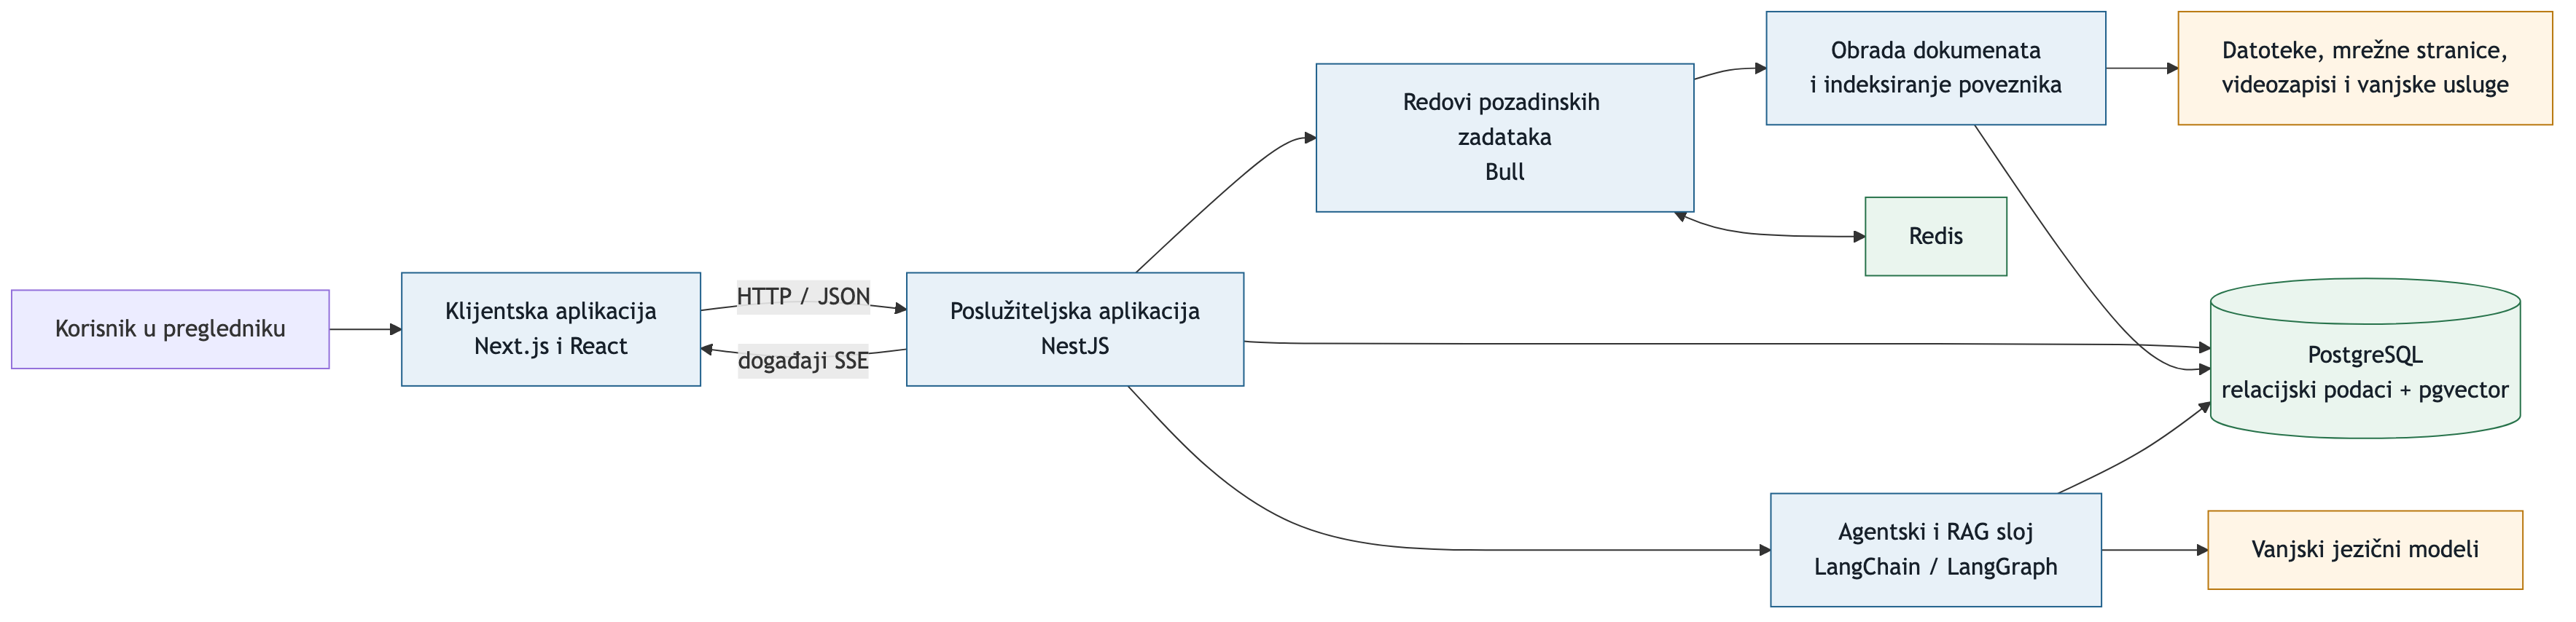
\includegraphics[width=\textwidth]{assets/arhitektura_sustava.png}
    \caption{Arhitektura razvijenog sustava}
    \label{fig:arhitektura-sustava}
\end{figure}

Agentski sloj i dohvat potpomognut generiranjem nalaze se u poslužiteljskoj aplikaciji. Agent prima pitanje, povijest razgovora i skup alata dopuštenih trenutačnom korisniku. Kada je za odgovor potrebno znanje iz prostora, alat za pretraživanje dohvaća indeksirane cjeline iz PostgreSQL-a i vraća ih zajedno s metapodacima izvora. Jezični model pritom ne pristupa bazi podataka izravno. Može zatražiti samo radnje koje mu je poslužiteljska aplikacija izložila, pa se provjera pristupa provodi prije dohvata, a granice prostora znanja ne ovise o odabranom modelu.

Dodatak~\ref{app:agentski-sustav} prikazuje programski kôd za sastavljanje agenta, odabir konfiguracije modela i pripremu konteksta razgovora. Iz tog je postupka vidljivo da se agent ne pokreće samo s korisničkim pitanjem. Uz pitanje dobiva alate i ovisnosti ograničene na trenutačnog korisnika i odabrani prostor znanja.

Za pohranu relacijskih podataka i vektorskih ugradnji koristi se PostgreSQL. Jedna baza čuva vezu između dokumenta, njegovih cjelina, prostora znanja i ovlasti preko stranih ključeva. Proširenje pgvector u istoj bazi omogućuje usporedbu vektora, pa semantički indeks nije izdvojen u zaseban sustav. Dio modela podataka koji sudjeluje u upravljanju znanjem prikazan je na slici~\ref{fig:model-baze-znanja}. Dijagram je izveden iz modela Prisma i ograničen na polja potrebna za razumijevanje toka sadržaja.

\begin{figure}[H]
    \centering
    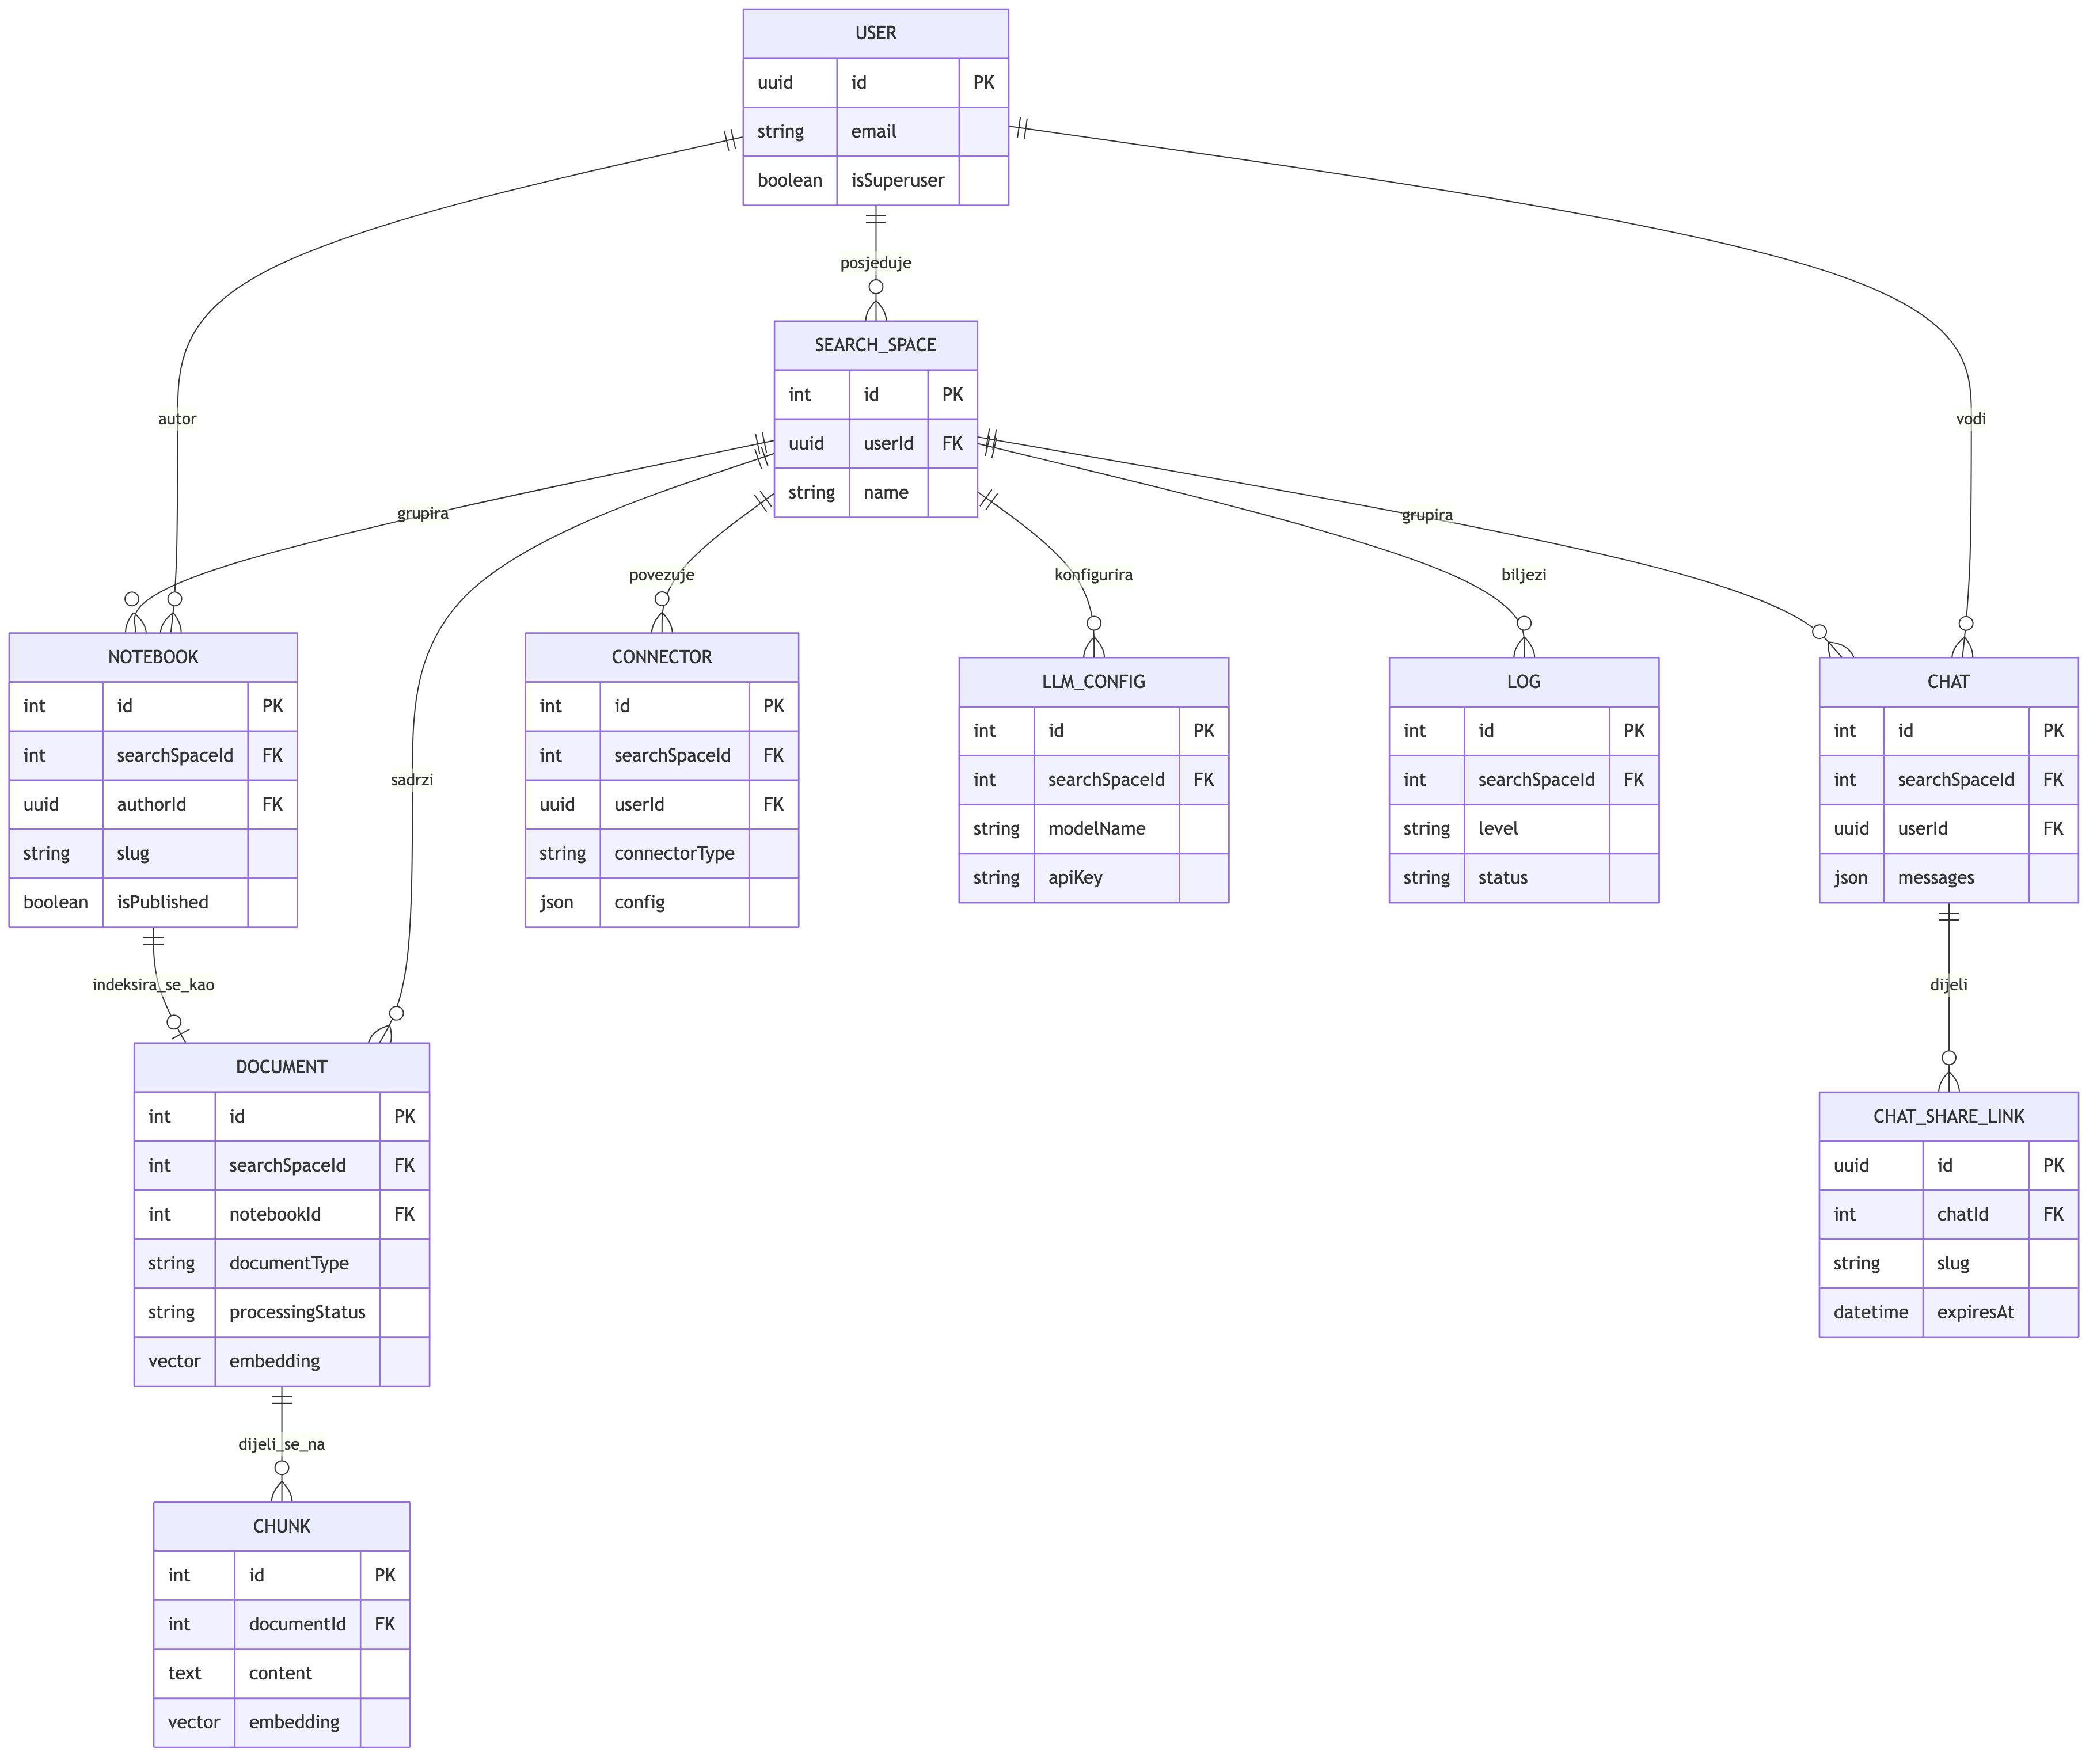
\includegraphics[width=0.92\textwidth]{assets/model_baze_znanja.png}
    \caption{Model podataka za prostore znanja, dokumente i razgovore}
    \label{fig:model-baze-znanja}
\end{figure}

Entitet \texttt{SearchSpace} povezuje dokumente, razgovore, bilježnice, poveznike, dnevnike i konfiguracije jezičnih modela. Svaki \texttt{Document} pripada jednom prostoru i čuva vrstu izvora, metapodatke i stanje obrade. Obrađeni sadržaj dijeli se na zapise \texttt{Chunk}, u kojima se uz tekst pohranjuje vektorska ugradnja. Zbog tog zajedničkog oblika datoteka, mrežna stranica, videozapis i zapis vanjske usluge mogu se pretraživati istim postupkom. Modelu se ne šalje cijeli dokument, nego samo cjeline povezane s korisničkim upitom.

Razgovor se povezuje s korisnikom i prostorom znanja kako bi se mogao nastaviti u istom kontekstu i prikazati u povijesti. Javna poveznica pohranjuje se odvojeno od razgovora te ima vlastitu oznaku, rok valjanosti i stanje aktivacije. Zbog toga dijeljenje ne otkriva unutarnji identifikator razgovora niti primatelju daje ovlasti za njegovo mijenjanje. Bilježnica se također pohranjuje kao zaseban sadržaj, ali se njezin tekst pri spremanju povezuje s dokumentom. Time objavljena ili privatna bilježnica može sudjelovati u pretraživanju istog prostora znanja.

Konfiguracija poveznika čuva podatke potrebne za pristup podržanoj vanjskoj usluzi te vrijeme posljednjeg i sljedećeg indeksiranja. Nakon dohvata zapisi se, neovisno o izvornom sustavu, pretvaraju u dokumente i cjeline opisane prethodnim modelom. Razgovorni dio sustava zato pretražuje jedinstveni indeks i ne mora poznavati posebnosti svake povezane usluge.

Podaci o članstvu, pozivnicama i potrošnji odvojeni su od sadržaja znanja. Njihov je odnos prikazan na slici~\ref{fig:model-pristupa}. Članstvo povezuje korisnika s prostorom i dodjeljuje mu ulogu vlasnika, urednika ili pregledavatelja. Vlasnik upravlja prostorom i članovima, urednik mijenja zajednički sadržaj, a pregledavatelj čita sadržaj i vodi vlastite razgovore. Pozivnica postoji samo do prihvaćanja ili isteka, nakon čega se za konkretnog korisnika stvara članstvo.

\begin{figure}[H]
    \centering
    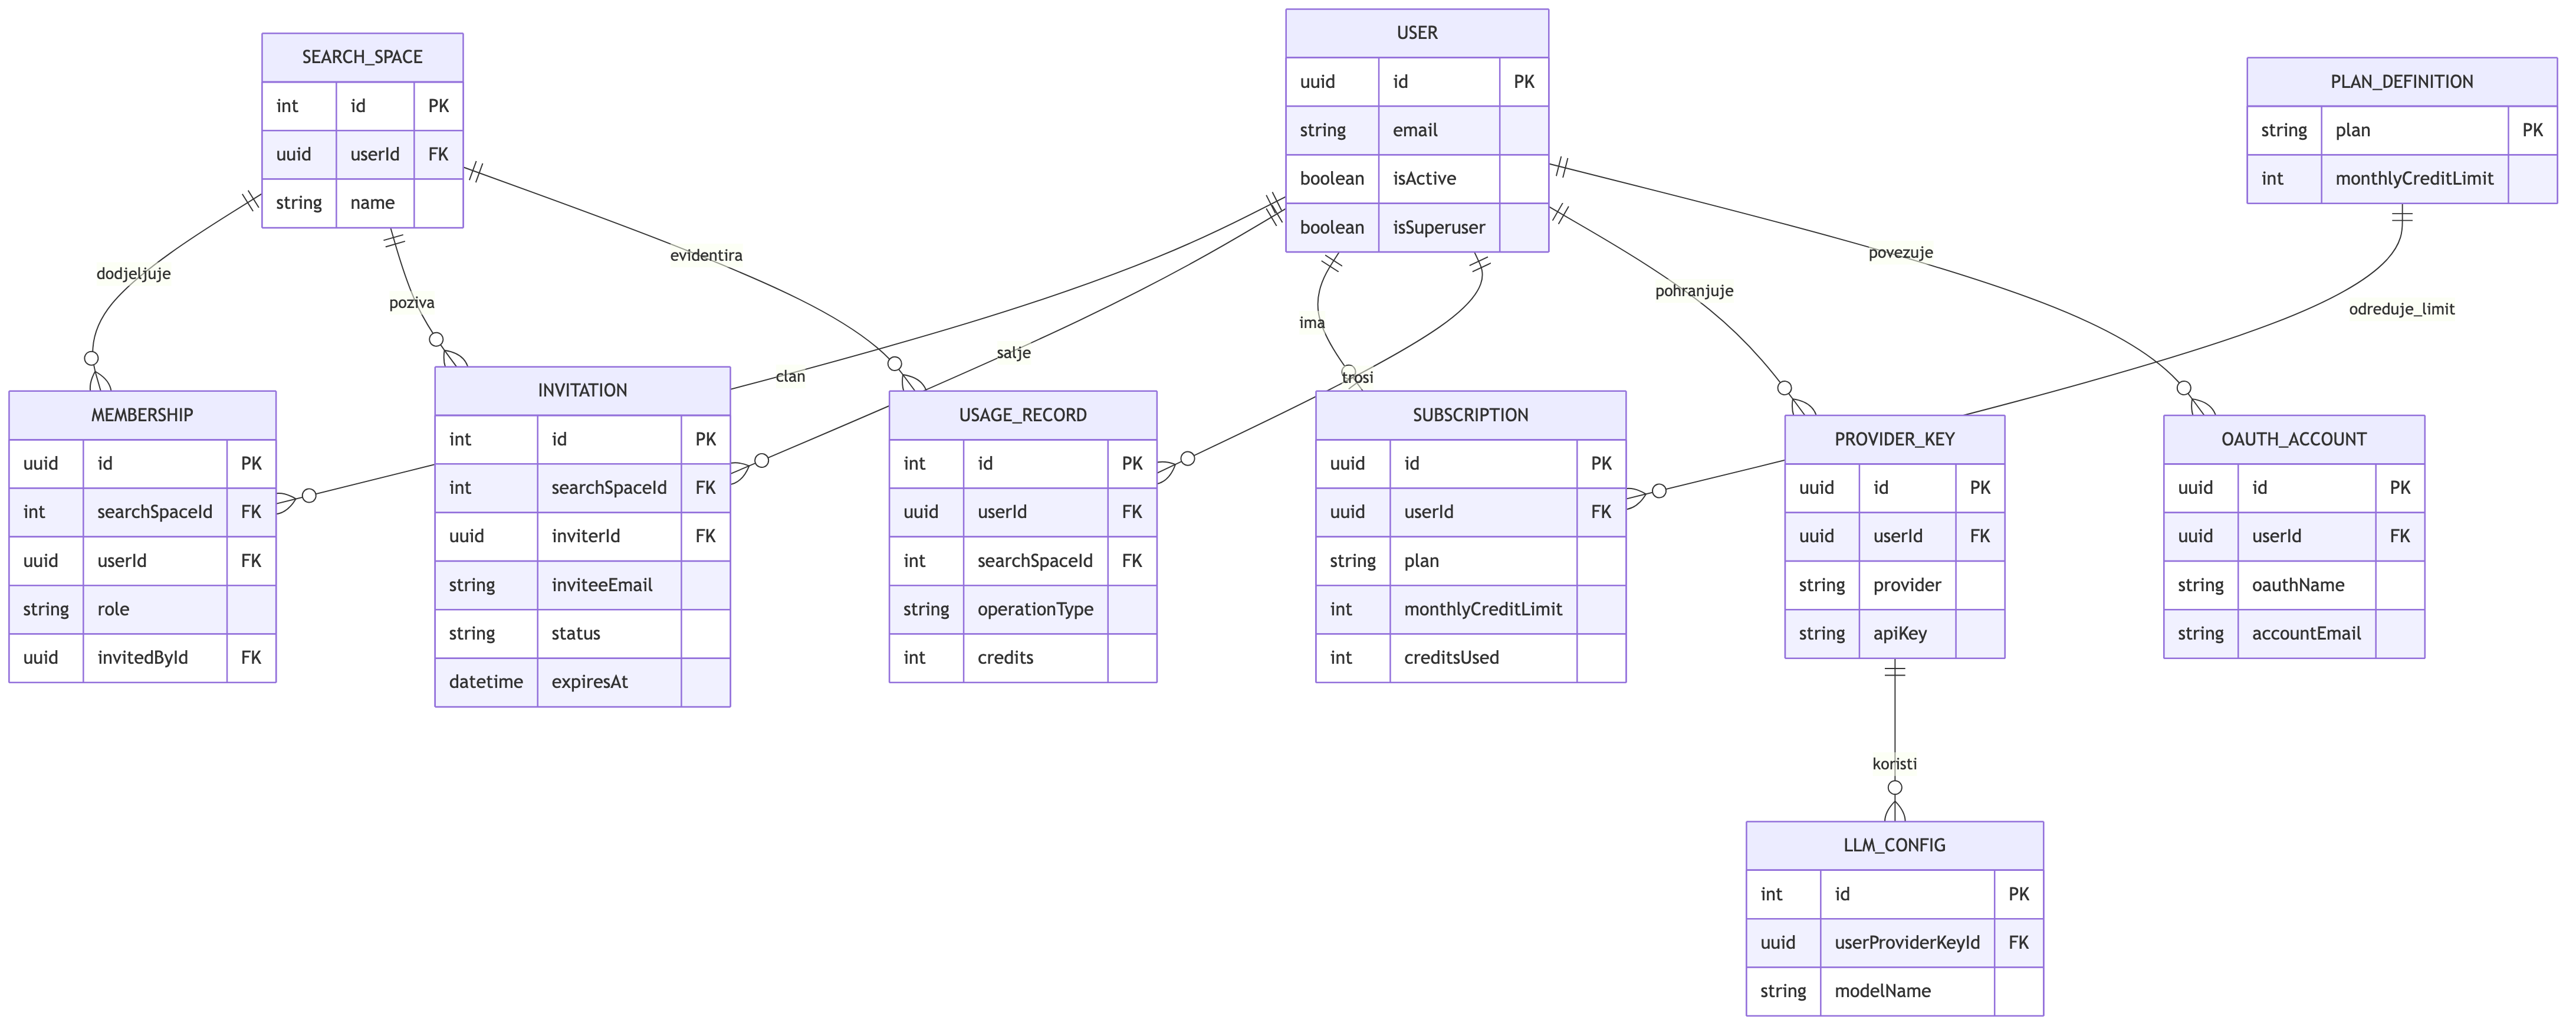
\includegraphics[width=\textwidth]{assets/model_pristupa_i_naplate.png}
    \caption{Model podataka za pristup prostorima, pretplate i potrošnju}
    \label{fig:model-pristupa}
\end{figure}

\DiffComment{str 14\newline "Skrivanje nedopuštenih radnji u korisničkom sučelju nije jedina zaštita."\newline a) odakle je sad palo (s neba) skrivanje nedopuštenih radnji koje do sad nije nigdje spomenuto?\newline b) odakle je sad pala (s neba) nekakva zaštita kad do sada nije nigdje spomenuta nikakva zaštita?\newline c) zaštita od čega?}
\DiffReplace{Skrivanje nedopuštenih radnji u korisničkom sučelju nije jedina zaštita. Za svaki zaštićeni zahtjev poslužiteljski čuvar provjerava članstvo i minimalnu potrebnu ulogu. Ako korisnik ne pripada prostoru ili nema potrebnu ovlast, zahtjev se prekida prije izvršavanja poslovne operacije. Isto se pravilo zato primjenjuje i kada je zahtjev poslan izravno poslužitelju, mimo korisničkog sučelja.}{Uloge određuju koje radnje korisničko sučelje nudi pojedinom članu prostora znanja. Primjerice, pregledavatelju nisu prikazane radnje za mijenjanje ili brisanje zajedničkog sadržaja. Takav prikaz sprječava neprimjerene radnje u uobičajenom radu, ali sam po sebi ne štiti dokumente i podatke od neovlaštenog pristupa. Zato poslužiteljski čuvar prije svake zaštićene operacije provjerava pripada li korisnik prostoru znanja i ima li najmanju potrebnu ulogu. Ako taj uvjet nije ispunjen, zahtjev se prekida prije čitanja ili izmjene podataka. Ista se provjera izvodi i kada je zahtjev poslan izravno poslužitelju, bez korisničkog sučelja.}

Pretplata je vezana uz korisnika, a ne uz pojedini prostor znanja. U njoj se čuvaju paket, mjesečno ograničenje i iskorišteni krediti, dok zaseban zapis potrošnje povezuje naplaćenu operaciju s korisnikom i prostorom. Takva podjela omogućuje prikaz ukupne potrošnje korisnika i naknadnu analizu po prostoru ili vrsti operacije. Definicije paketa izdvojene su od pojedinačnih pretplata kako bi se ograničenja mogla mijenjati bez promjene programskog kôda.

Opisani model uspostavlja tri granice koje se ponavljaju u ostatku aplikacije. Sadržaj je razdvojen po prostorima znanja, ovlasti su određene članstvom, a potrošnja korisničkom pretplatom. Isti korisnik zato može imati različite uloge u različitim prostorima, dok se dokumenti, razgovori i konfiguracije modela uvijek obrađuju u kontekstu odabranog prostora.

\section{Izgled korisničkog sučelja i funkcionalnosti sustava}

\DiffComment{str 14\newline "Neregistrirani korisnik pristupa autentifikaciji i namjerno objavljenom sadržaju."\newline Možda ne razumijem, ali kakav bi to bio nenamjerno objavljen sadržaj i koja je razlika u ovom kontekstu?}
\DiffReplace{Korisničko sučelje slijedi granice opisane u modelu podataka. Javni dio služi prijavi, registraciji i čitanju namjerno objavljenog sadržaja. Nakon prijave korisnik bira prostor znanja, a sučelje prikazuje radnje dopuštene njegovom članstvu. Administratorske stranice izdvojene su iz tog tijeka jer se odnose na cijelu platformu, a ne na pojedini prostor.}{Korisničko sučelje slijedi granice opisane u modelu podataka. Javni dio omogućuje prijavu i registraciju te čitanje bilježnica koje je njihov autor izričito objavio za javnost. Svi ostali dokumenti, razgovori i privatne bilježnice ostaju dostupni samo članovima pripadajućeg prostora znanja. Nakon prijave korisnik bira prostor znanja, a sučelje prikazuje radnje dopuštene njegovom članstvu. Administratorske stranice izdvojene su iz tog tijeka jer se odnose na cijelu platformu, a ne na pojedini prostor.}

\subsection{Aplikacija namijenjena neregistriranim korisnicima}

\DiffComment{riječ autentifikacija potrebno je promijeniti u autentikacija -\newline autentikacija ima engleske korijene, a autentifikacija francuske.}
Neregistrirani korisnik najprije dolazi do granice između javnog i privatnog dijela sustava. Može se prijaviti adresom elektroničke pošte i lozinkom, upotrijebiti Google račun ili otvoriti postupak registracije. Obrasci za prijavu i registraciju prikazani su na slikama~\ref{fig:prijava} i~\ref{fig:registracija}. Odvojeni obrasci jasno označavaju prijelaz u privatne prostore znanja, a poveznica za povratak na prijavu povezuje oba postupka u isti \DiffReplaceInline{autentifikacijski}{autentikacijski} tijek.

\begin{figure}[H]
    \centering
    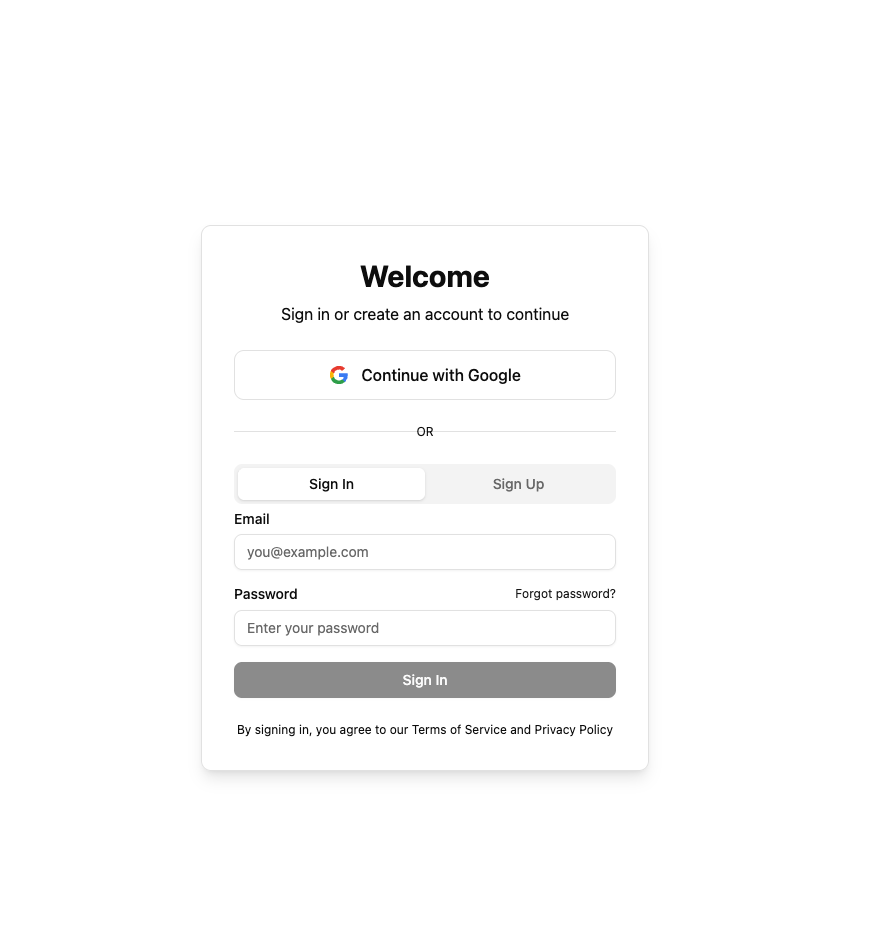
\includegraphics[width=0.9\textwidth,height=0.72\textheight,keepaspectratio]{assets/ui/login.png}
    \caption{Prijava korisnika adresom elektroničke pošte ili Google računom}
    \label{fig:prijava}
\end{figure}

\begin{figure}[H]
    \centering
    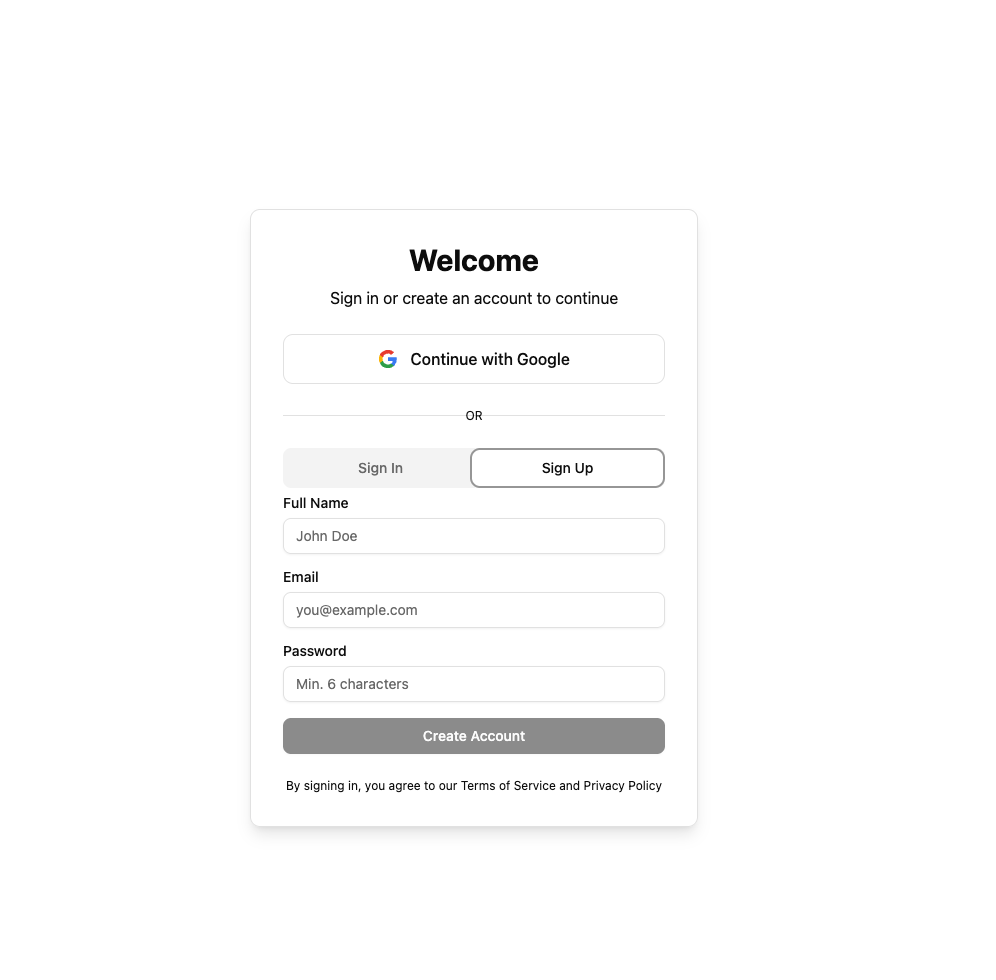
\includegraphics[width=0.9\textwidth,height=0.72\textheight,keepaspectratio]{assets/ui/registracija.png}
    \caption{Registracija novog korisničkog računa}
    \label{fig:registracija}
\end{figure}

\DiffComment{str 16\newline "primiti uputu"...\newline kakvu uputu? Mislim znam, ali pojasnite.\newline\newline str 16\newline "Poslužitelj izrađuje vremenski ograničenu oznaku"\newline - što točno poslužitelj izrađuje? Vi ste to programirali, objasnite detaljnije.\newline\newline str 16\newline "Jednaka poruka nakon predaje zahtjeva"\newline Jednaka u odnosu na što i koga? Znam, ali pojasnite.}
\DiffReplace{Postupak oporavka lozinke mora pomoći korisniku, ali ne smije otkrivati podatke o tuđem računu. Zato korisnik u obrascu na slici~\ref{fig:zaboravljena-lozinka} unosi adresu elektroničke pošte na koju želi primiti uputu. Poslužitelj izrađuje vremenski ograničenu oznaku, pa se nova lozinka može postaviti samo dok je poveznica valjana. Nakon predaje zahtjeva prikazuje se ista poruka bez obzira na to postoji li unesena adresa u sustavu.}{Postupak oporavka lozinke mora pomoći korisniku, ali ne smije otkrivati postoji li tuđi korisnički račun. Korisnik u obrascu na slici~\ref{fig:zaboravljena-lozinka} unosi svoju adresu elektroničke pošte i, ako je povezana s računom koji koristi lozinku, prima poruku s poveznicom za postavljanje nove lozinke. Poslužitelj za taj zahtjev nasumično generira heksadecimalnu oznaku za ponovno postavljanje lozinke, sprema je uz korisnički račun i određuje joj rok valjanosti od jednog sata. Oznaka je dio poveznice iz poruke, a poslužitelj pri postavljanju nove lozinke provjerava odgovara li spremljenoj oznaci i je li rok još valjan. Nakon slanja obrasca korisniku se uvijek prikazuje poruka da je poruka za oporavak poslana: ista poruka prikazuje se i za postojeću i za nepostojeću adresu. Time se iz odgovora ne može zaključiti je li određena adresa registrirana u aplikaciji.}

\begin{figure}[H]
    \centering
    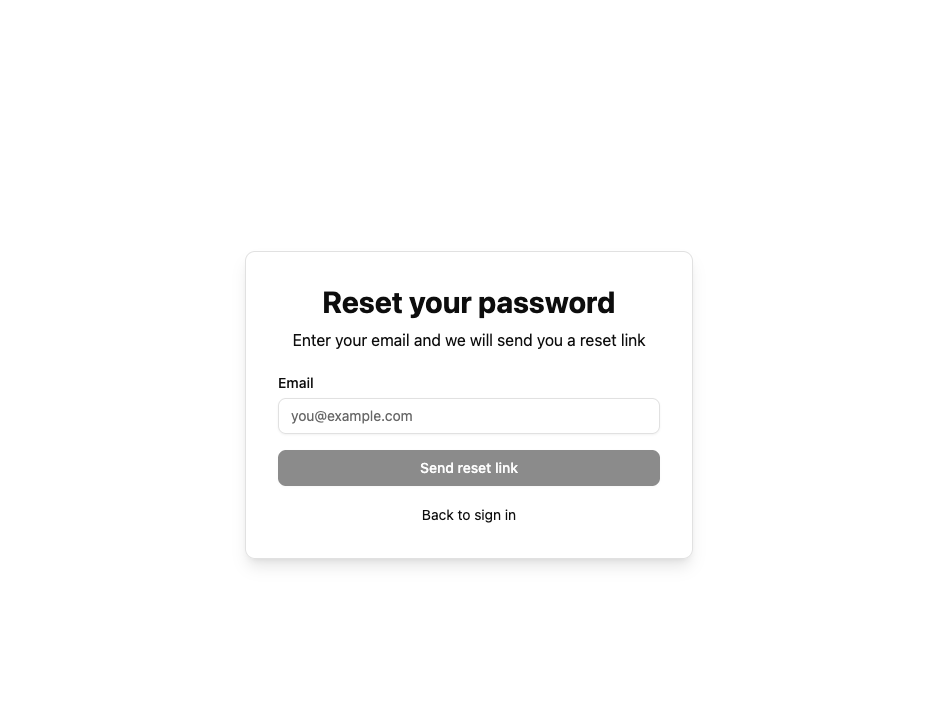
\includegraphics[width=0.9\textwidth,height=0.72\textheight,keepaspectratio]{assets/ui/zaboravljena_lozinka.png}
    \caption{Zahtjev za ponovno postavljanje zaboravljene lozinke}
    \label{fig:zaboravljena-lozinka}
\end{figure}

\DiffComment{riječ autentifikacija potrebno je promijeniti u autentikacija -\newline autentikacija ima engleske korijene, a autentifikacija francuske.}
Nakon uspješne prijave klijent dohvaća podatke trenutačnog korisnika i preusmjerava ga prema dostupnim prostorima znanja. \DiffReplaceInline{Autentifikacijski}{Autentikacijski} postupak time završava određivanjem korisničkog konteksta, a ne samo provjerom vjerodajnica.

Javni dio sustava nije samo uvod u prijavu. Dio sadržaja namjerno ostaje dostupan bez korisničkog računa. Objavljene bilježnice imaju ulogu blogova: mogu se pretraživati prema naslovu, poredati prema datumu objave i otvoriti putem javne oznake \texttt{slug}. Javni prikaz ne izlaže ostali sadržaj prostora znanja. Sličan se princip primjenjuje na podijeljeni razgovor. Njegova poveznica omogućuje samo čitanje, može imati rok valjanosti i može se opozvati. Pozivnicu za članstvo neregistrirani korisnik može otvoriti, ali je prihvaća tek nakon prijave kako bi se članstvo povezalo s određenim računom.

Javni popis i pojedinačna objava prikazani su na slici~\ref{fig:javni-sadrzaj}. Pretraživanje i sortiranje olakšavaju pronalaženje objave, dok zaseban javni prikaz potvrđuje da čitatelj dobiva pristup odabranom sadržaju, a ne cijelom prostoru znanja.

\begin{figure}[H]
    \centering
    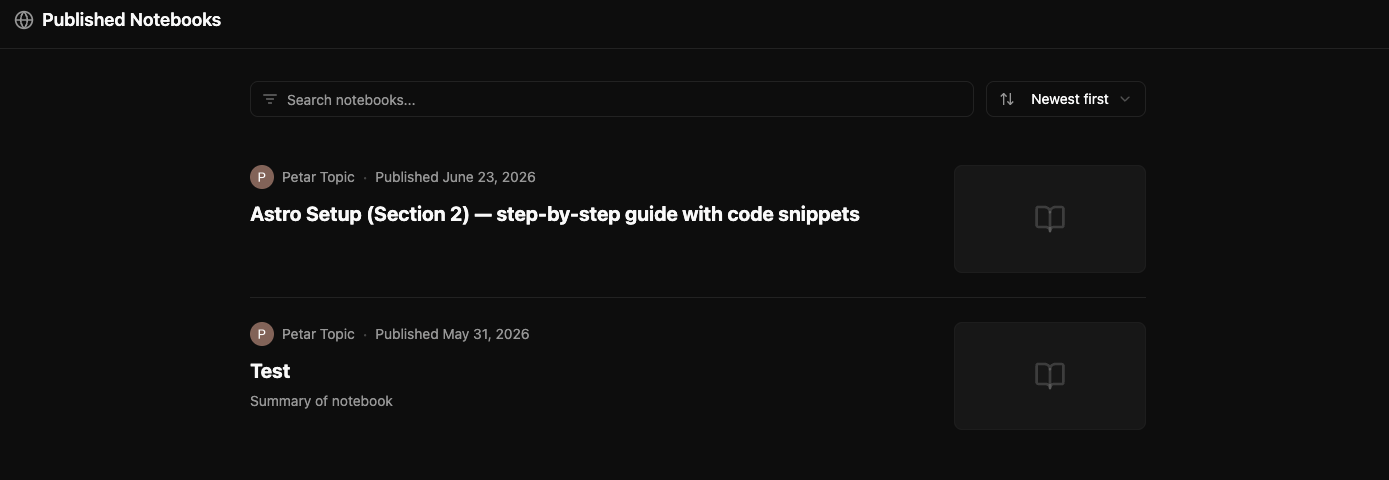
\includegraphics[width=0.95\textwidth,height=0.72\textheight,keepaspectratio]{assets/ui/javne_biljeznjice.png}
    \caption{Javno pretraživanje i čitanje objavljenih bilježnica}
    \label{fig:javni-sadrzaj}
\end{figure}

\subsection{Aplikacija namijenjena registriranim korisnicima}

Nakon prijave korisnik najprije bira kontekst rada. Može otvoriti postojeći prostor znanja ili stvoriti novi. Pri stvaranju unosi naziv, opis i po želji naslovnu sliku, a sustav mu automatski dodjeljuje ulogu vlasnika. Vlasnik naknadno može promijeniti osnovne podatke i sliku ili izbrisati prostor. Ostalim članovima te su radnje dostupne samo kada ih dopušta dodijeljena uloga. Odabrani prostor zatim postaje kontekst za dokumente, razgovore, bilježnice i poveznike, čime se sprječava miješanje sadržaja različitih baza znanja.

Obrazac na slici~\ref{fig:uredivanje-prostora} objedinjuje stvaranje i uređivanje osnovnih podataka prostora. Ista struktura obrasca smanjuje razliku između početnog unosa i kasnije izmjene, dok je brisanje izdvojeno kao radnja dostupna vlasniku.

\begin{figure}[H]
    \centering
    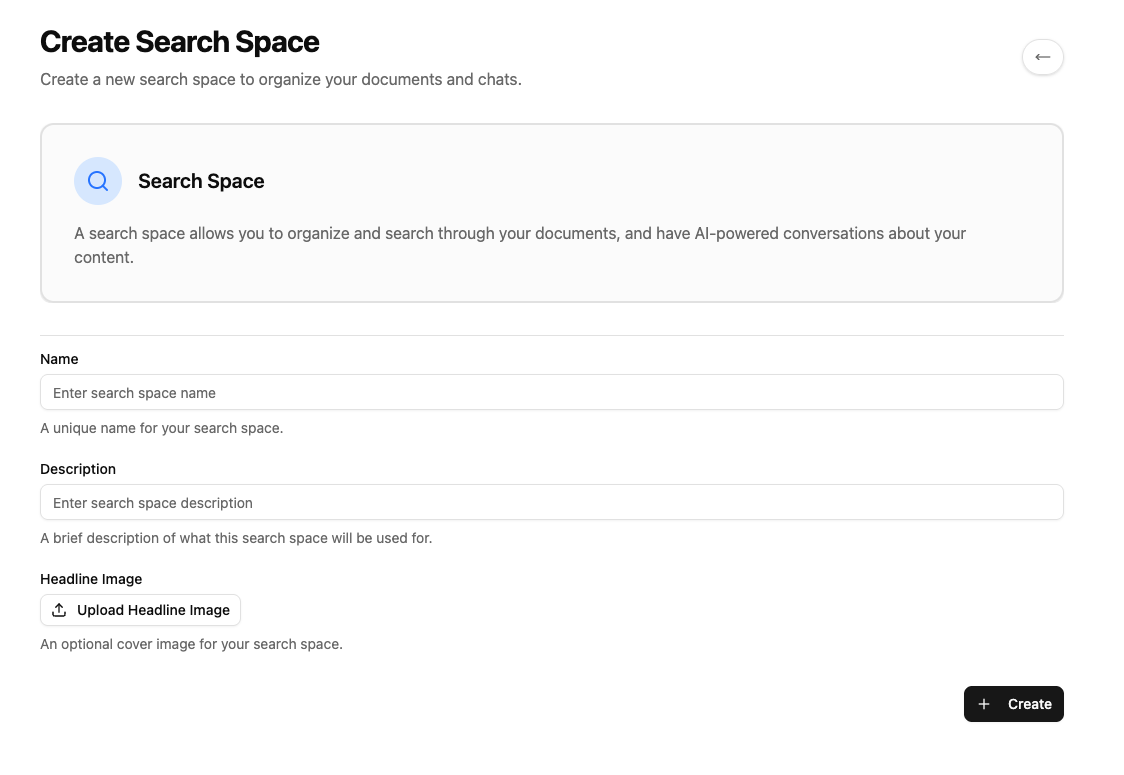
\includegraphics[width=0.95\textwidth,height=0.72\textheight,keepaspectratio]{assets/ui/stvaranje_prostora_znanja.png}
    \caption{Stvaranje i uređivanje prostora znanja}
    \label{fig:uredivanje-prostora}
\end{figure}

Pregled dostupnih prostora prikazan je na slici~\ref{fig:prostori-znanja}. Pretraživanje prema naslovu omogućuje pronalaženje prostora bez pregledavanja cijelog popisa, a prikaz uloge objašnjava zašto se raspoložive radnje mogu razlikovati među prostorima istog korisnika.

\begin{figure}[H]
    \centering
    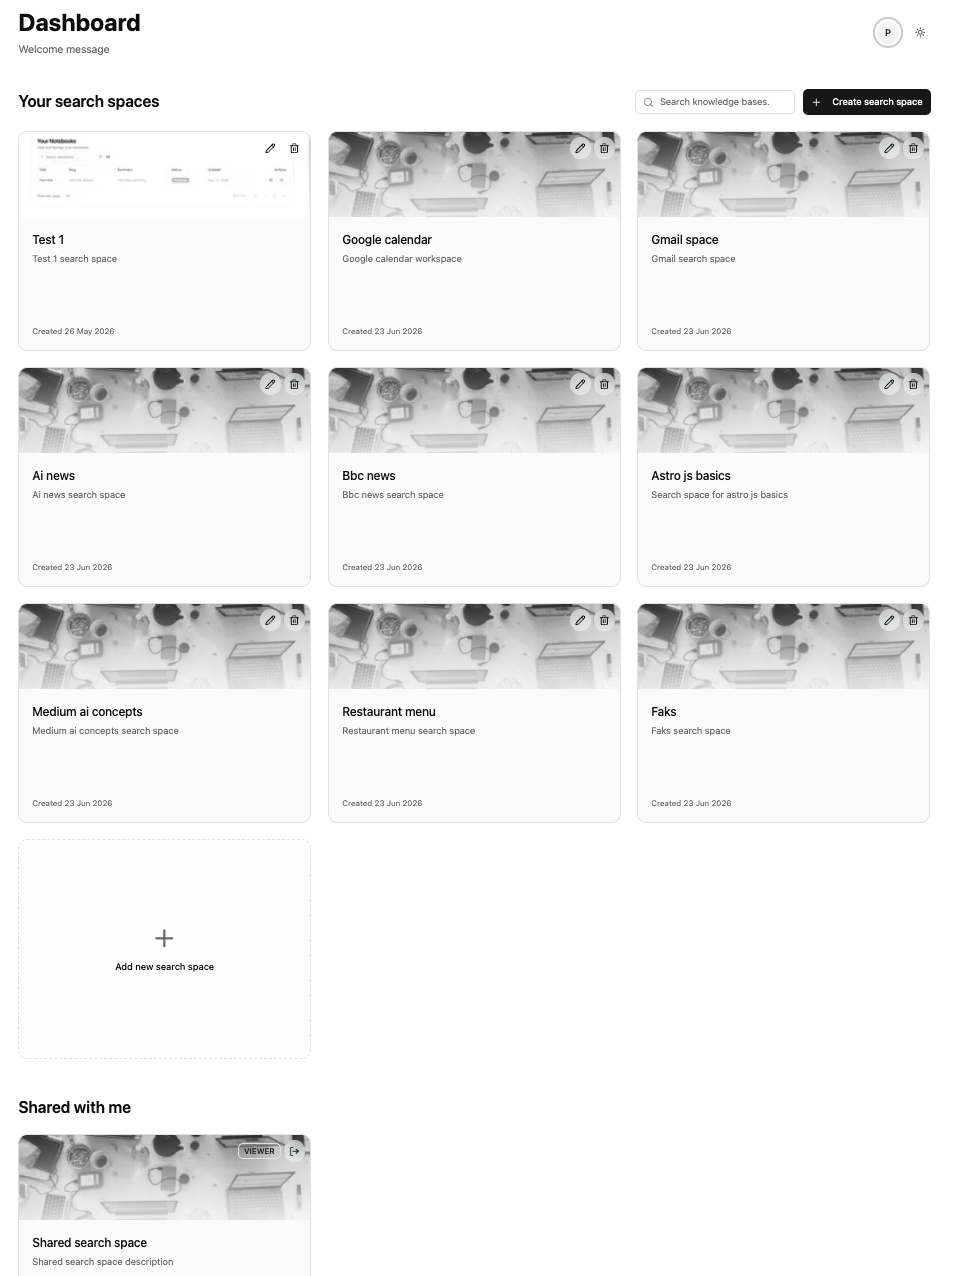
\includegraphics[width=0.95\textwidth,height=0.72\textheight,keepaspectratio]{assets/ui/pregled_prostora_znanja.png}
    \caption{Pregled prostora znanja dostupnih prijavljenom korisniku}
    \label{fig:prostori-znanja}
\end{figure}

Kada je prostor odabran, sljedeći je korak unos izvora. Vlasnik ili urednik može prenijeti datoteku, unijeti adresu mrežne stranice, dodati videozapis s platforme YouTube ili povezati podržanu vanjsku uslugu. Ručni unos prikladan je za pojedinačne izvore, dok su poveznici namijenjeni sadržaju koji već nastaje u drugim sustavima. Poveznici za Slack, Notion, GitHub, Google Calendar i Gmail dohvaćaju takav sadržaj bez ručnog prijenosa svake stavke. Spremljene konfiguracije mogu se pretraživati prema nazivu, mijenjati i uklanjati.

Popis poveznika na slici~\ref{fig:poveznici} razlikuje dostupne vrste usluga od već konfiguriranih izvora. Prikaz stanja i radnji upravljanja omogućuje korisniku da utvrdi koji se vanjski sadržaj uključuje u odabrani prostor znanja.

\begin{figure}[H]
    \centering
    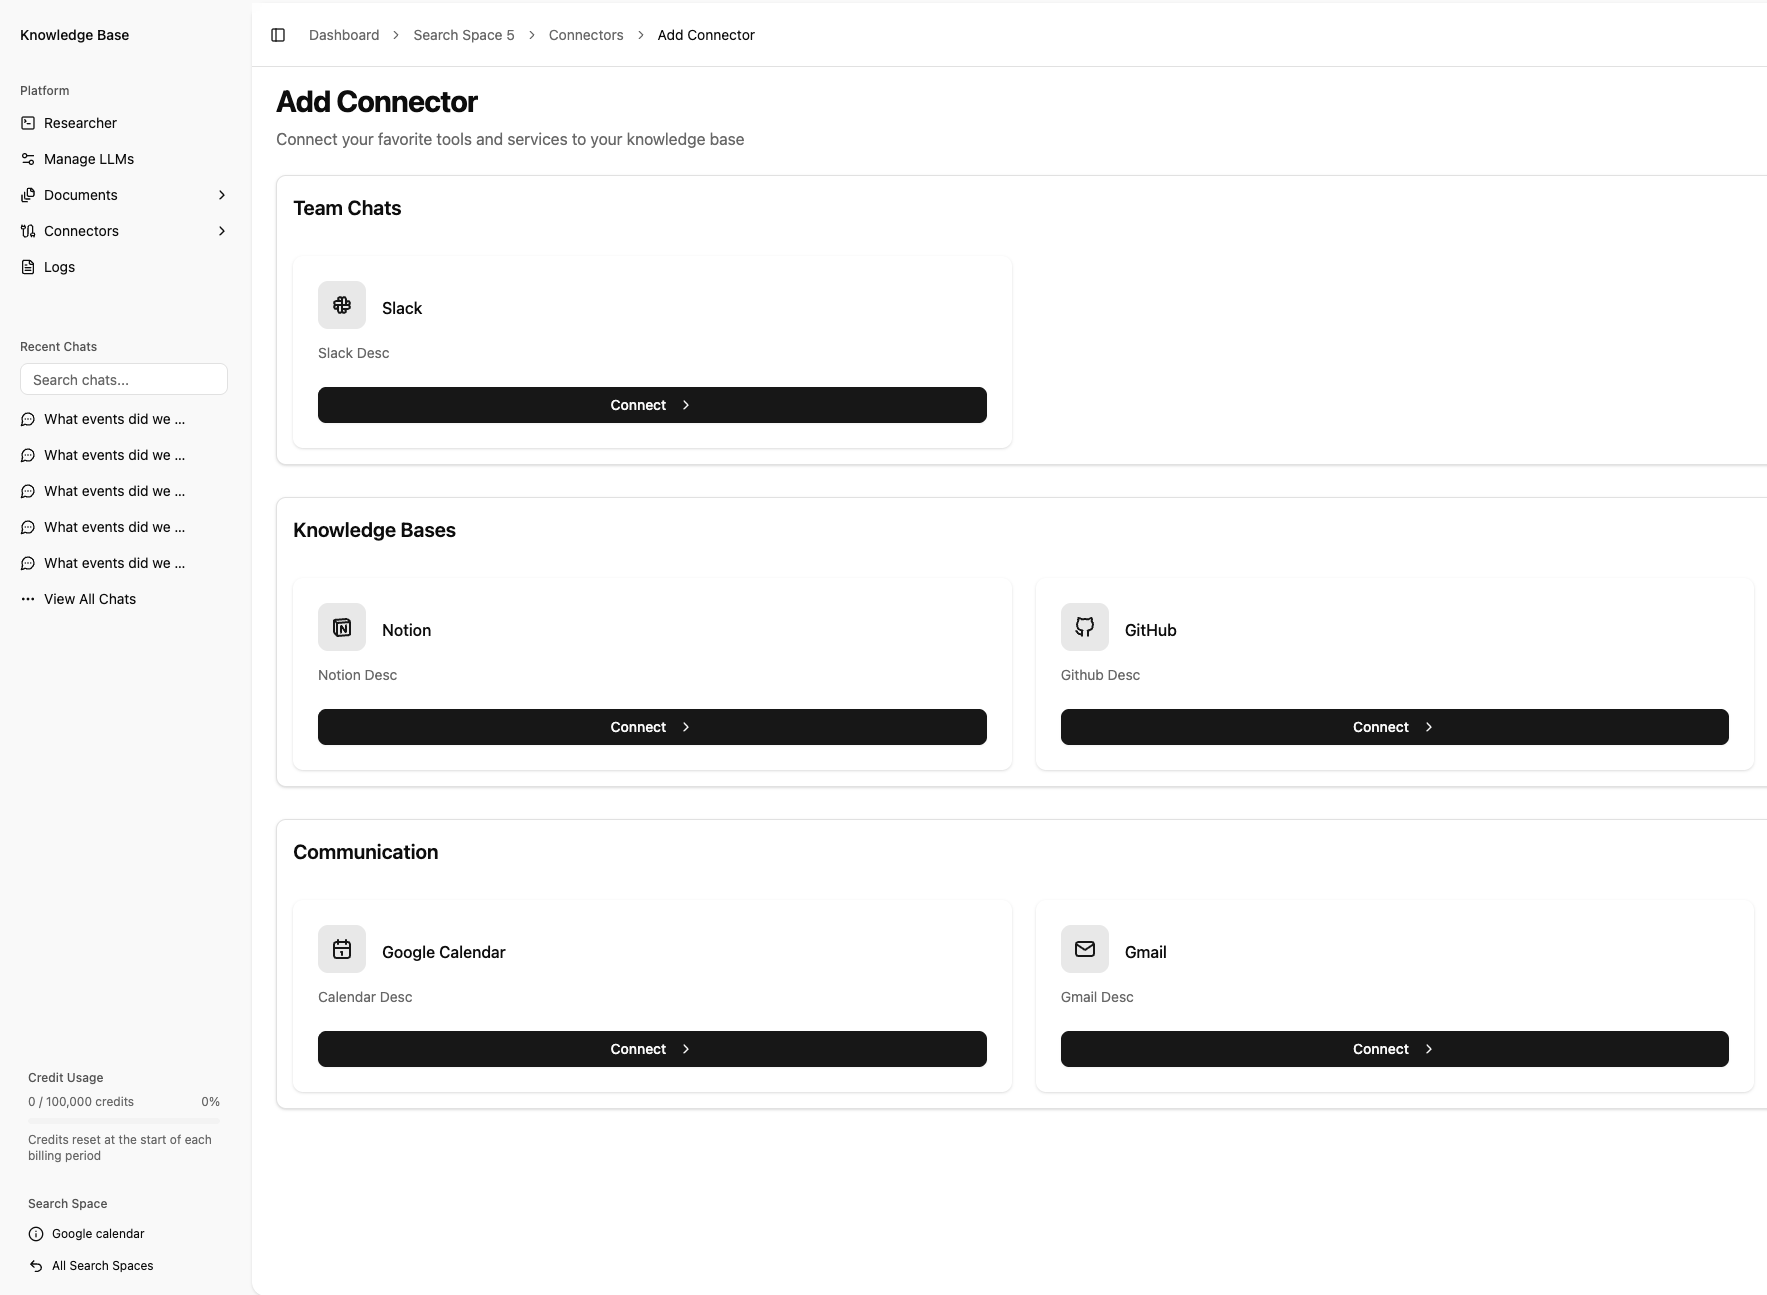
\includegraphics[width=0.95\textwidth,height=0.72\textheight,keepaspectratio]{assets/ui/prikaz_dostupnih_poveznika.png}
    \caption{Odabir i upravljanje poveznicima vanjskih izvora}
    \label{fig:poveznici}
\end{figure}

Vanjski izvor može sadržavati mnogo zapisa, pa korisnik prije indeksiranja određuje opseg obrade. Može zadati vremenski raspon, pokrenuti brzo osvježavanje ili uključiti periodičku obradu. Brzo osvježavanje nastavlja od posljednjeg uspješnog indeksiranja, a kada takav podatak ne postoji, dohvaća sadržaj iz prethodne godine. Periodički način koristi spremljeni sljedeći termin kako bi poslužiteljski planer predao novi zadatak u red i nakon završetka izračunao iduće izvođenje. Tako se početni unos većeg opsega sadržaja odvaja od redovitog održavanja indeksa.

Postavke opsega i učestalosti prikazane su na slici~\ref{fig:indeksiranje-poveznika}. Odabrane vrijednosti određuju količinu sadržaja koja ulazi u zadatak i trenutak njegova ponovnog izvođenja.

\begin{figure}[H]
    \centering
    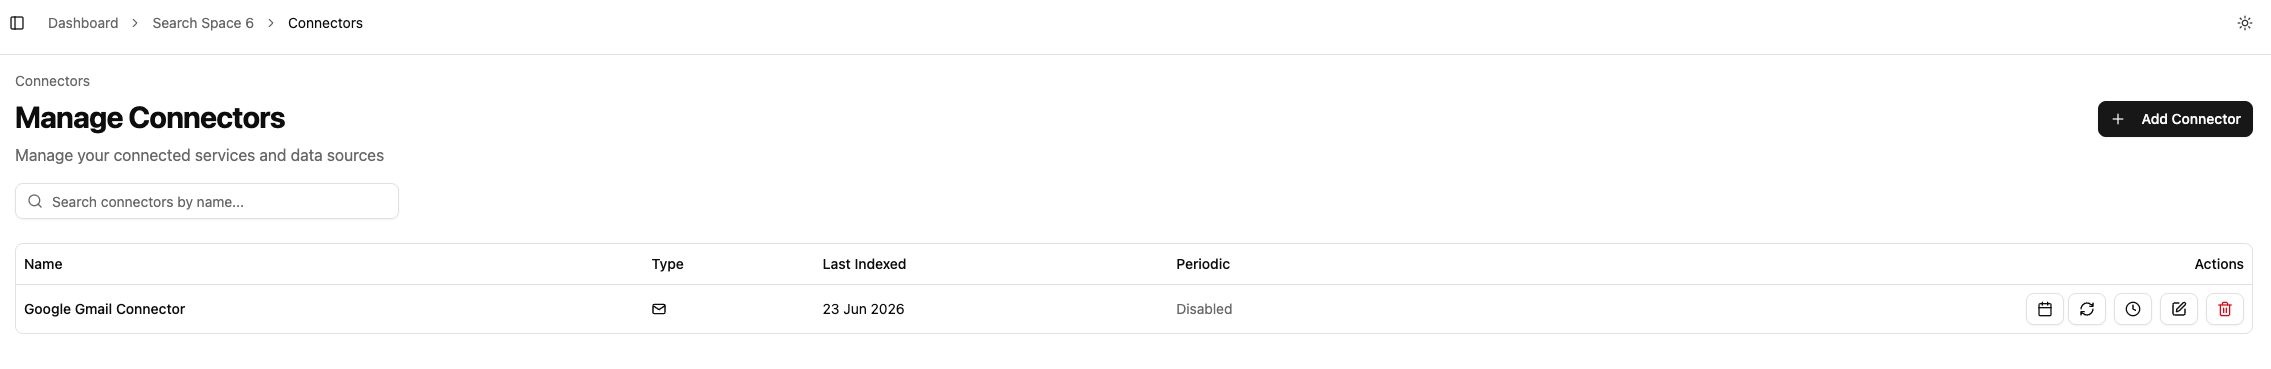
\includegraphics[width=0.95\textwidth,height=0.72\textheight,keepaspectratio]{assets/ui/postavljeni_poveznici.png}
    \caption{Postavljanje opsega i rasporeda indeksiranja poveznika}
    \label{fig:indeksiranje-poveznika}
\end{figure}

\DiffComment{str 22\newline - na slici se vidi mogućnost uploada videa (mp4...), nigdje u radu to ne spominjete, samo Youtube}
\DiffReplace{Neposredni unos izvora ima jednostavniji tijek, ali se obrazac prilagođava vrsti sadržaja. Prijenos datoteke prikazan je na slici~\ref{fig:prijenos-dokumenta}, unos mrežne stranice na slici~\ref{fig:indeksiranje-stranice}, a dodavanje videozapisa s platforme YouTube na slici~\ref{fig:indeksiranje-youtubea}. Sva tri postupka završavaju stvaranjem dokumenta u istom prostoru znanja. Razlikuje se samo početni način izdvajanja sadržaja.}{Neposredni unos izvora ima jednostavniji tijek, ali se obrazac prilagođava vrsti sadržaja. Prijenos datoteke prikazan je na slici~\ref{fig:prijenos-dokumenta}; uz dokumente i slike može obuhvatiti i lokalno spremljene videozapise u formatima \texttt{.mp4}, \texttt{.mpeg} i \texttt{.webm}. Unos mrežne stranice prikazan je na slici~\ref{fig:indeksiranje-stranice}. Videozapis s platforme YouTube dodaje se zasebnim obrascem na slici~\ref{fig:indeksiranje-youtubea}, u koji korisnik unosi njegovu mrežnu adresu. Sva tri postupka završavaju stvaranjem dokumenta u istom prostoru znanja. Razlikuje se samo početni način izdvajanja sadržaja.}

\begin{figure}[H]
    \centering
    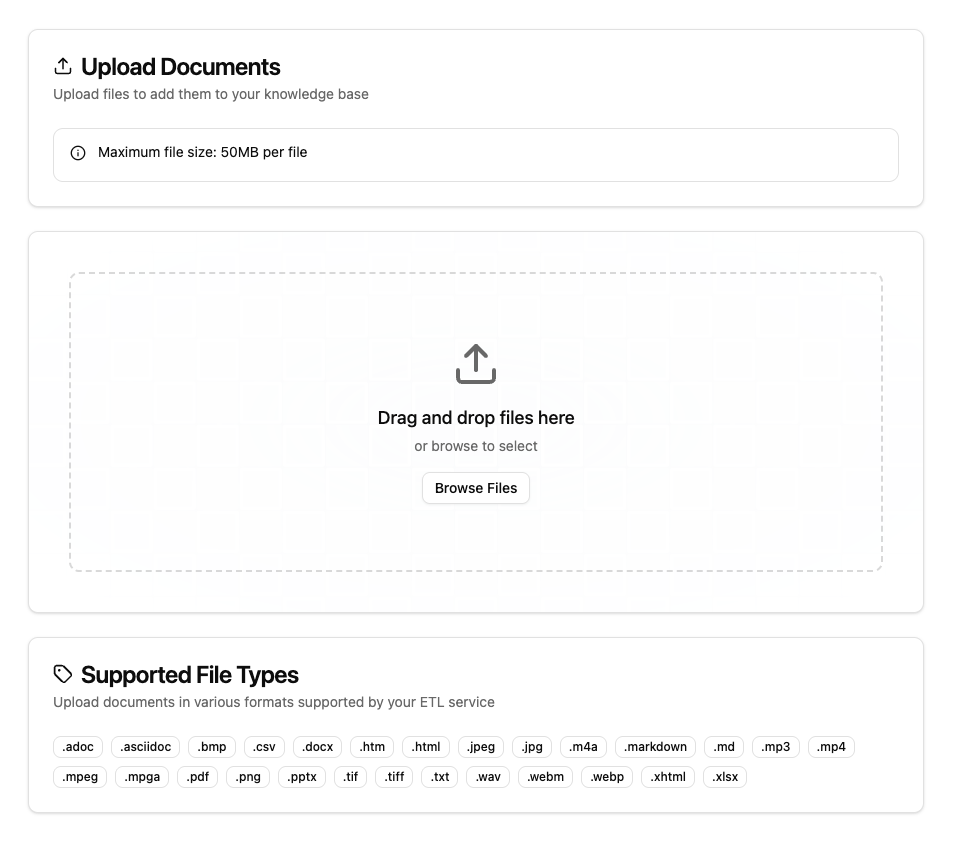
\includegraphics[width=0.9\textwidth,height=0.72\textheight,keepaspectratio]{assets/ui/prijenos_dokumenta.png}
    \caption{Prijenos dokumenta u prostor znanja}
    \label{fig:prijenos-dokumenta}
\end{figure}

\DiffComment{str 22\newline - na slici se nekakav ETL service koji nije objašnjen u tekstu}
\DiffAdd{U ovom sustavu naziv ETL servis označava pozadinsku komponentu koja obrađuje prenesenu datoteku prije indeksiranja. Ovisno o konfiguraciji koristi se Docling ili LlamaCloud. Odabrani servis iz datoteke izdvaja sadržaj i vraća Markdown tekst s metapodacima, uključujući podatke o stranicama kada su dostupni. Poslužiteljska aplikacija zatim iz tog rezultata stvara dokument, dijeli tekst na cjeline i za svaku cjelinu izrađuje vektorsku ugradnju. Oznaka 	extit{Supported File Types} na slici zato prikazuje formate koje odabrani ETL servis može obraditi.}

\begin{figure}[H]
    \centering
    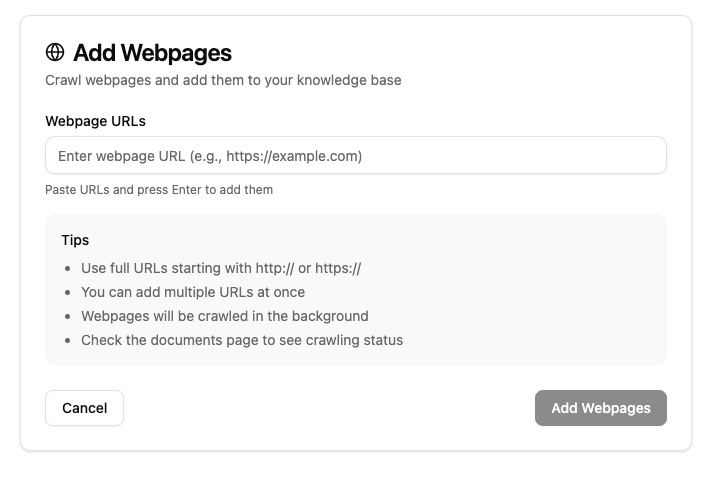
\includegraphics[width=0.9\textwidth,height=0.72\textheight,keepaspectratio]{assets/ui/prijenos_mrezne_stranice.png}
    \caption{Dodavanje i indeksiranje mrežne stranice}
    \label{fig:indeksiranje-stranice}
\end{figure}

\begin{figure}[H]
    \centering
    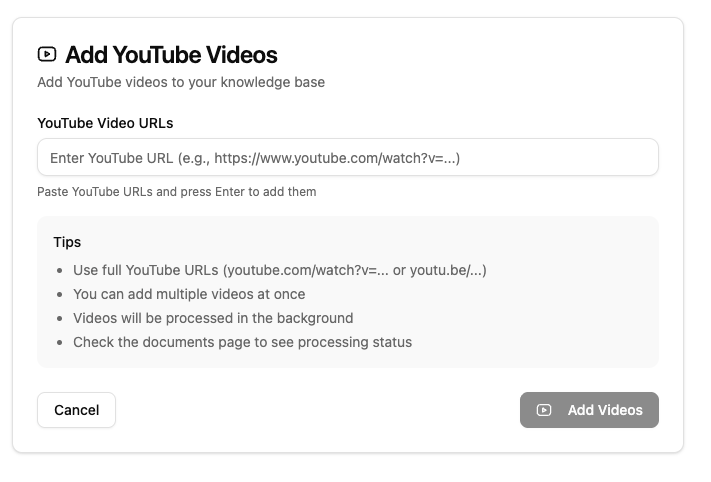
\includegraphics[width=0.9\textwidth,height=0.72\textheight,keepaspectratio]{assets/ui/prijenos_youtube_videa.png}
    \caption{Dodavanje i indeksiranje videozapisa YouTube}
    \label{fig:indeksiranje-youtubea}
\end{figure}

Nakon predaje izvor još nije spreman za razgovor. Poslužitelj najprije stvara zapis sa stanjem \texttt{PROCESSING} i zadatak predaje pozadinskom procesu. Tijekom obrade izdvaja se sadržaj, analiziraju pronađene slike, tekst i slikovni opisi dijele se na cjeline te se za svaku cjelinu izrađuje vektorska ugradnja. Slike iz datoteka i mrežnih stranica tako mogu sudjelovati u kasnijem dohvatu putem prepoznatog teksta, opisa ili sadržaja grafikona. Uspješno izvršavanje mijenja stanje u \texttt{COMPLETED}, a pogreška u \texttt{FAILED}. Događaji SSE prenose promjenu klijentu, pa korisnik ne mora ručno osvježavati popis dokumenata.

\DiffComment{str 24\newline "radnik" > što je to na engleskom jeziku? U kodu u dodatku nisam prepoznao što bi to bilo. Provjerite i budite jasniji/uskladite terminologiju hr/en/nazivi\_funkcija u kodu}
\DiffReplace{Dodatak~\ref{app:indeksiranje-dokumenata} prikazuje podjelu sadržaja prema njegovoj strukturi te izradu vektorske ugradnje za svaku dobivenu cjelinu. Predavanje datoteke u red i radnik koji provodi obradu prikazani su u dodatku~\ref{app:pozadinski-zadaci}. Odvajanjem tih postupaka zahtjev za prijenos može završiti prije dugotrajnog izdvajanja i indeksiranja sadržaja, dok radnik zasebno bilježi uspjeh ili pogrešku.}{Dodatak~\ref{app:indeksiranje-dokumenata} prikazuje podjelu sadržaja prema njegovoj strukturi te izradu vektorske ugradnje za svaku dobivenu cjelinu. Predavanje datoteke u red i njezina obrada prikazani su u dodatku~\ref{app:pozadinski-zadaci}. Zadatak iz reda preuzima procesorska klasa \texttt{DocumentsProcessor} (engl. \textit{processor}); njezina metoda \texttt{processFileDocument} poziva \texttt{processFileInBackground}, koja izdvaja i indeksira sadržaj prenesene datoteke. Odvajanjem tih postupaka zahtjev za prijenos može završiti prije dugotrajne obrade, dok procesor zasebno bilježi uspjeh ili pogrešku.}

Nakon obrade korisniku treba pregled izvora, ali i način provjere što je stvarno indeksirano. Popis dokumenata pokriva prvi dio tog zadatka. Zapisi se mogu pretraživati prema naslovu, filtrirati, sortirati i pregledavati po stranicama. Vidljivi se stupci mogu prilagoditi, a omiljeni dokumenti izdvojiti iz ostatka popisa. Vlasnik ili urednik može ukloniti jedan dokument ili skup odabranih zapisa, dok se nedopuštene radnje ne prikazuju pregledavatelju. Otvaranjem dokumenta korisnik prelazi sa sažetog stanja obrade na sadržaj koji je pripremljen za pretraživanje.

Detaljni prikaz dokumenta na slici~\ref{fig:detalji-dokumenta} objedinjuje sažetak, metapodatke i nastale cjeline. Taj prikaz omogućuje provjeru sadržaja dostupnog pretraživanju i objašnjava iz kojeg dijela izvora kasnije nastaje citat u razgovoru.

\begin{figure}[H]
    \centering
    
\includegraphics[width=0.9\textwidth,height=0.72\textheight,keepaspectratio]{assets/ui/detalji_dokumenta.png}
    \caption{Pregled metapodataka i cjelina obrađenog dokumenta}
    \label{fig:detalji-dokumenta}
\end{figure}

\DiffComment{str 25\newline Kakav je to Jina Crawler u screenshotu? Nema ga u radu.}
\DiffAdd{Polje \texttt{Crawler Type: Jina Reader} na slici označava servis Jina Reader, uključen u poslužiteljski dio aplikacije. Nakon što korisnik unese mrežnu adresu, servis Jina Reader dohvaća sadržaj te stranice i vraća ga kao Markdown tekst s metapodacima. Dobiveni tekst zatim prolazi isti postupak podjele na cjeline i izrade vektorskih ugradnji kao i prenesene datoteke.}

Stranica za upravljanje dokumentima prikazana je na slici~\ref{fig:upravljanje-dokumentima}. Vrsta izvora i stanje uz svaki zapis povezuju asinkronu obradu s povratnom informacijom u sučelju, dok pretraživanje, filtri i radnje omogućuju upravljanje većim brojem dokumenata.

\begin{figure}[H]
    \centering
    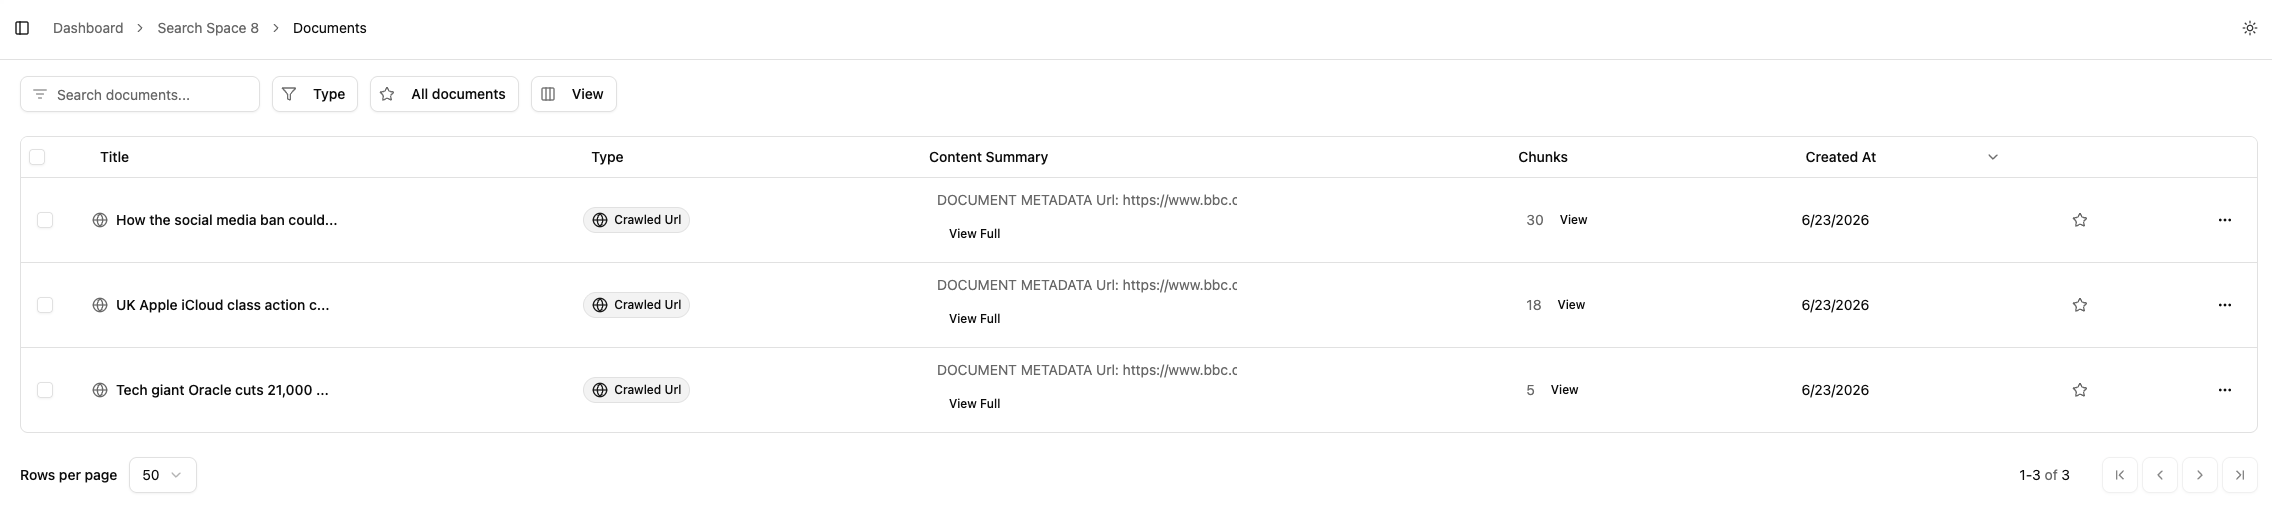
\includegraphics[width=0.95\textwidth,height=0.72\textheight,keepaspectratio]{assets/ui/upravljanje_dokumentima.png}
    \caption{Upravljanje dokumentima i prikaz stanja njihove obrade}
    \label{fig:upravljanje-dokumentima}
\end{figure}

Dnevnici su drugi pogled na isti pozadinski rad. Dokument prikazuje rezultat obrade pojedinog izvora, a dnevnik pokazuje tijek i ishod zadataka. Popis se može pretraživati prema sadržaju poruke, filtrirati, sortirati i pregledavati po stranicama, a vidljivi se stupci mogu prilagoditi. Otvaranjem zapisa prikazuju se cijela poruka i metapodaci potrebni za utvrđivanje izvora pogreške. Zapisi se mogu ukloniti pojedinačno ili skupnim odabirom. Sažetak posljednja 24 sata prikazuje ukupan broj zapisa, aktivne zadatke, broj neuspjeha i udio uspješnih izvršavanja. Novi zapisi i promjene postojećih prenose se događajima SSE, pa pregled prati izvođenje bez ručnog osvježavanja.

Sažetak i tablica dnevnika prikazani su na slici~\ref{fig:dnevnici-obrade}. Zbirni pokazatelji daju pregled stanja obrade, dok pojedinačni zapisi omogućuju prelazak na poruku i metapodatke konkretnog zadatka.

\begin{figure}[H]
    \centering
    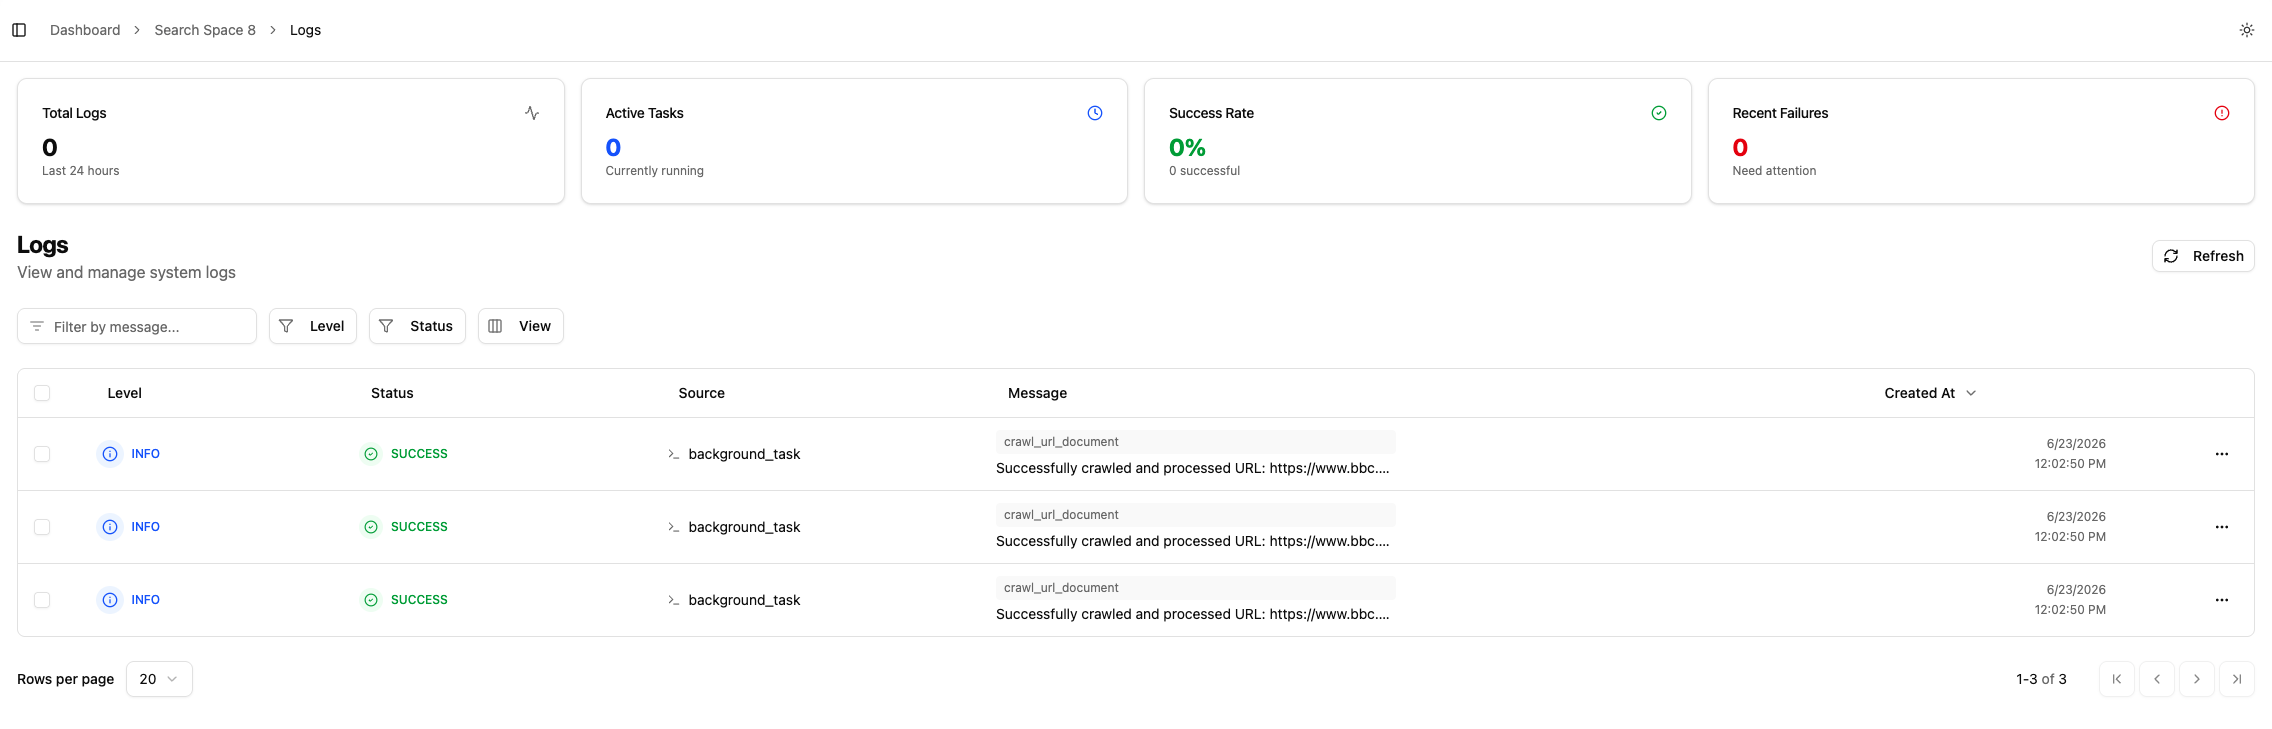
\includegraphics[width=0.95\textwidth,height=0.72\textheight,keepaspectratio]{assets/ui/prikaz_dnevnika.png}
    \caption{Praćenje ishoda pozadinske obrade u dnevnicima prostora}
    \label{fig:dnevnici-obrade}
\end{figure}

Tek nakon što su izvori pripremljeni, razgovor s bazom znanja postaje glavni način korištenja prostora. Agent prema potrebi poziva alat za hibridno pretraživanje. Pronađene se cjeline ponovno rangiraju i prosljeđuju modelu s oznakama izvora. Odgovor se prenosi postupno, pa korisnik vidi njegov nastanak prije završetka cijelog postupka. Svaki citat zadržava identifikator cjeline iz koje je izveden, zbog čega se iz odgovora može otvoriti naslov dokumenta, poveznica i izvorni ulomak.

\DiffReplace{Dodatak~\ref{app:hibridno-pretrazivanje} prikazuje programski kôd koji izrađuje ugradnju upita, neovisno rangira semantička i tekstualna podudaranja te ih spaja postupkom recipročnog fuzioniranja rangova. Uvjeti korisnika i prostora primjenjuju se prije dohvata, pa u rangiranje ne ulaze cjeline izvan dopuštenog konteksta.}{Dodatak~\ref{app:hibridno-pretrazivanje} prikazuje programski kôd koji izrađuje ugradnju upita te sastavlja dva poretka rezultata: semantički i tekstualni. Za svaku cjelinu postupak RRF računa doprinos \(1/(60+r)\) iz svakog poretka u kojem se pojavljuje, pri čemu je \(r\) njezin položaj na tom popisu. Doprinosi se zbrajaju, pa cjelina koja je među prvim rezultatima i semantičkog i tekstualnog pretraživanja ima veći konačni rezultat od cjeline koja je visoko rangirana samo u jednom poretku. Uvjeti korisnika i prostora primjenjuju se prije dohvata, pa u rangiranje ne ulaze cjeline izvan dopuštenog konteksta.}

Završeni odgovor i otvoreni izvor prikazani su na slici~\ref{fig:razgovor-citati}. Istodobna vidljivost pitanja, odgovora, oznaka citata i izvornog ulomka pokazuje da razgovorno sučelje ne skriva postupak dohvata, nego korisniku omogućuje provjeru korištenog konteksta.

\begin{figure}[H]
    \centering
    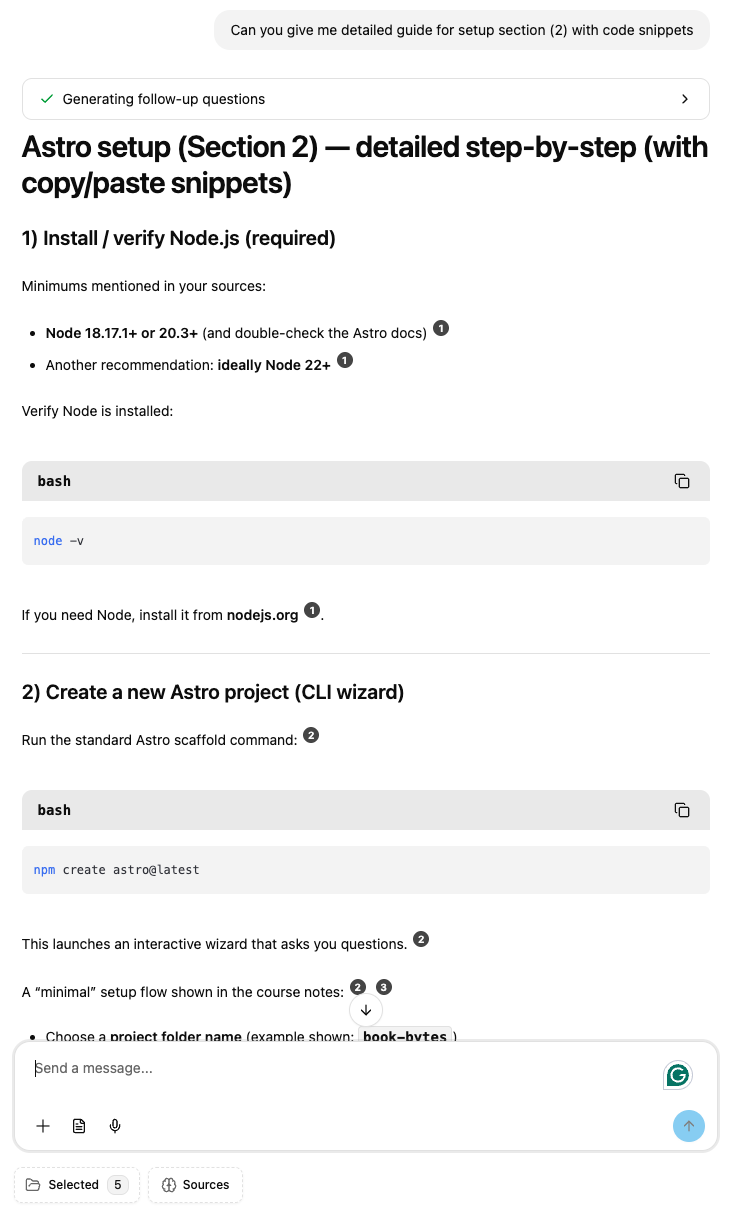
\includegraphics[width=0.9\textwidth,height=0.72\textheight,keepaspectratio]{assets/ui/prikaz_razgovora_s_agentom.png}
    \caption{Razgovor s bazom znanja i pregled izvora citiranog u odgovoru}
    \label{fig:razgovor-citati}
\end{figure}

Razgovor ne mora uvijek koristiti cijeli prostor znanja. Korisnik ga može ograničiti na odabrane dokumente ili mu pridružiti novu datoteku ili sliku. Datoteka, mrežna stranica ili videozapis mogu se poslati na indeksiranje izravno iz razgovora, bez prethodnog otvaranja popisa dokumenata. Agent raspolaže alatima za analizu slike te u odgovor može uključiti relevantne slike pronađene u izvorima. Jezik odgovora preuzima se iz aktivne konfiguracije modela i primjenjuje na sve upite u prostoru. Predlošci za sažetak, akcijski plan ili tehničku analizu pripremaju početni oblik zahtjeva, ali korisnik njihov sadržaj može izmijeniti prije slanja.

Primjer odgovora sa slikovnim sadržajem prikazan je na slici~\ref{fig:slikovni-odgovor}. Veza između korisničkog pitanja, slike, tekstualnog tumačenja i izvora razlikuje stvarnu uporabu slike od običnog prikaza privitka.

\begin{figure}[H]
    \centering
    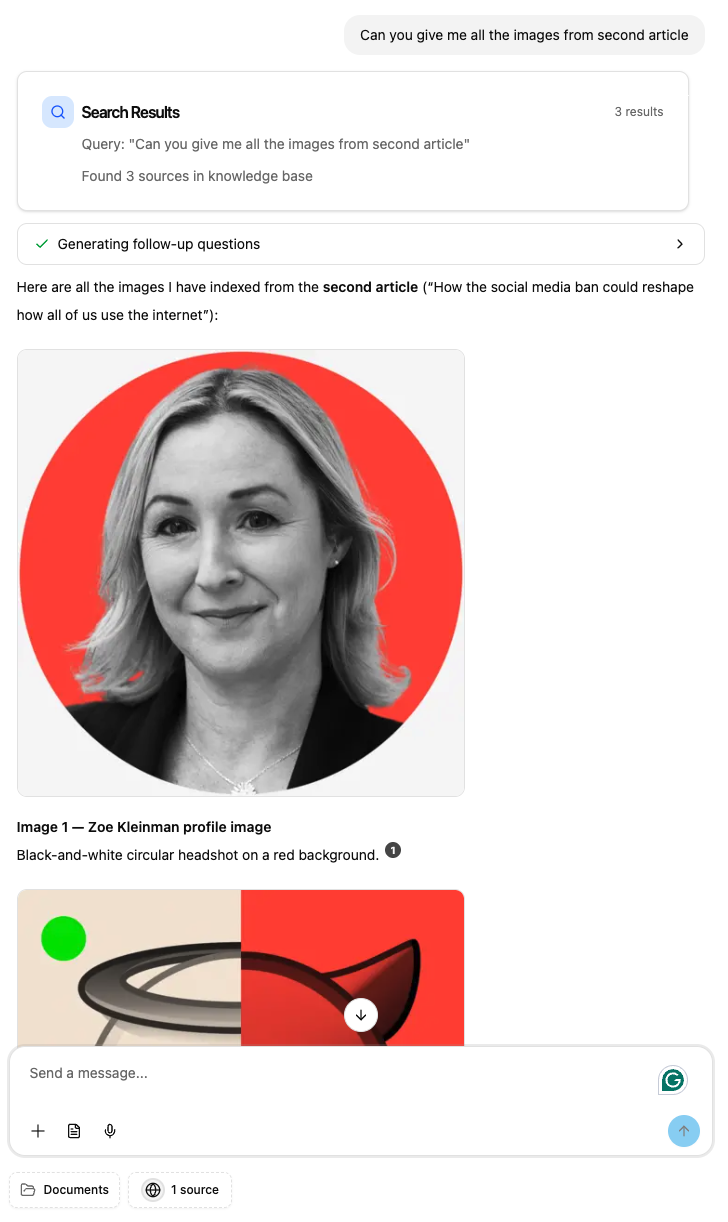
\includegraphics[width=0.9\textwidth,height=0.72\textheight,keepaspectratio]{assets/ui/prikaz_razgovora_s_agentom_s_analizom_slika.png}
    \caption{Analiza slikovnog sadržaja i prikaz relevantne slike u odgovoru}
    \label{fig:slikovni-odgovor}
\end{figure}

Izbornik predložaka i pripremljeni tekst poruke prikazani su na slici~\ref{fig:predlosci-upita}. Predložak ubrzava oblikovanje ponavljajućih zahtjeva, ali ne uvodi novi tip razgovora niti ograničava slobodan unos.

\begin{figure}[H]
    \centering
    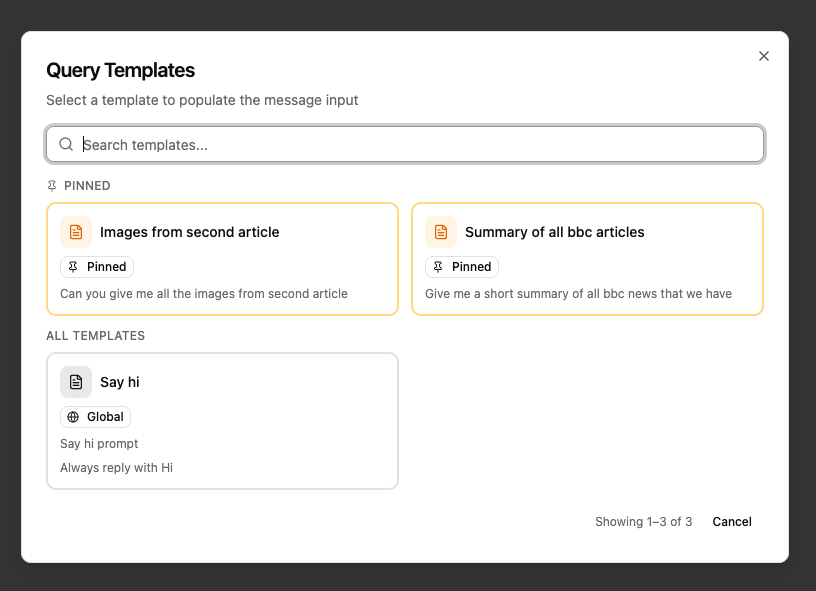
\includegraphics[width=0.9\textwidth,height=0.72\textheight,keepaspectratio]{assets/ui/predlozak_upita.png}
    \caption{Odabir predloška za oblikovanje korisničkog upita}
    \label{fig:predlosci-upita}
\end{figure}

Razgovor se često nastavlja kroz više koraka, pa se prethodni rad mora moći pronaći i urediti. Povijest razgovora može se pretraživati prema naslovu, filtrirati, sortirati i pregledavati po stranicama. Korisnik može promijeniti naslov, označiti razgovor kao omiljen ili ukloniti jedan odnosno više odabranih zapisa. Uređivanjem ranije poruke i ponovnim pokretanjem upita odgovor se gradi iz izmijenjenog tijeka. Ponovno pokretanje neizmijenjenog upita služi dobivanju novog odgovora u istom kontekstu. Vlasnik razgovora može izraditi javnu poveznicu samo za čitanje i naknadno je opozvati.

Pregled povijesti i postavke dijeljenja prikazani su na slici~\ref{fig:povijest-razgovora}. Popis služi privatnom upravljanju razgovorima, dok javna poveznica izlaže samo odabrani zapis bez ovlasti za njegovo mijenjanje.

\begin{figure}[H]
    \centering
    
\includegraphics[width=0.9\textwidth,height=0.72\textheight,keepaspectratio]{assets/ui/dijeljenje_razgovora.png}
    \caption{Upravljanje poviješću i dijeljenjem razgovora}
    \label{fig:povijest-razgovora}
\end{figure}

Nije svaki zapis prikladan za oblik razgovora. Zbog toga sustav ima bilježnice, namijenjene uređenom sadržaju koji korisnik želi spremiti, dopunjavati ili javno objaviti. U uređivaču obogaćenog teksta korisnik stvara strukturirani zapis, dodaje slike, pregledava spremljenu verziju i po potrebi je objavljuje putem javne poveznice. Bilježnica zadržava vezu s autorom i prostorom znanja. Pri spremanju se njezin sadržaj indeksira kao dokument, a nakon izmjene ponovno se obrađuje. Agent zato može pretraživati dopuštene bilježnice istim postupkom kao datoteke i vanjske izvore.

Popis bilježnica na slici~\ref{fig:popis-biljeznica} prikazuje status objave i radnje dostupne za svaki zapis. Korisnik tako prije otvaranja uređivača može razlikovati skicu od javno dostupnog sadržaja.

\begin{figure}[H]
    \centering
    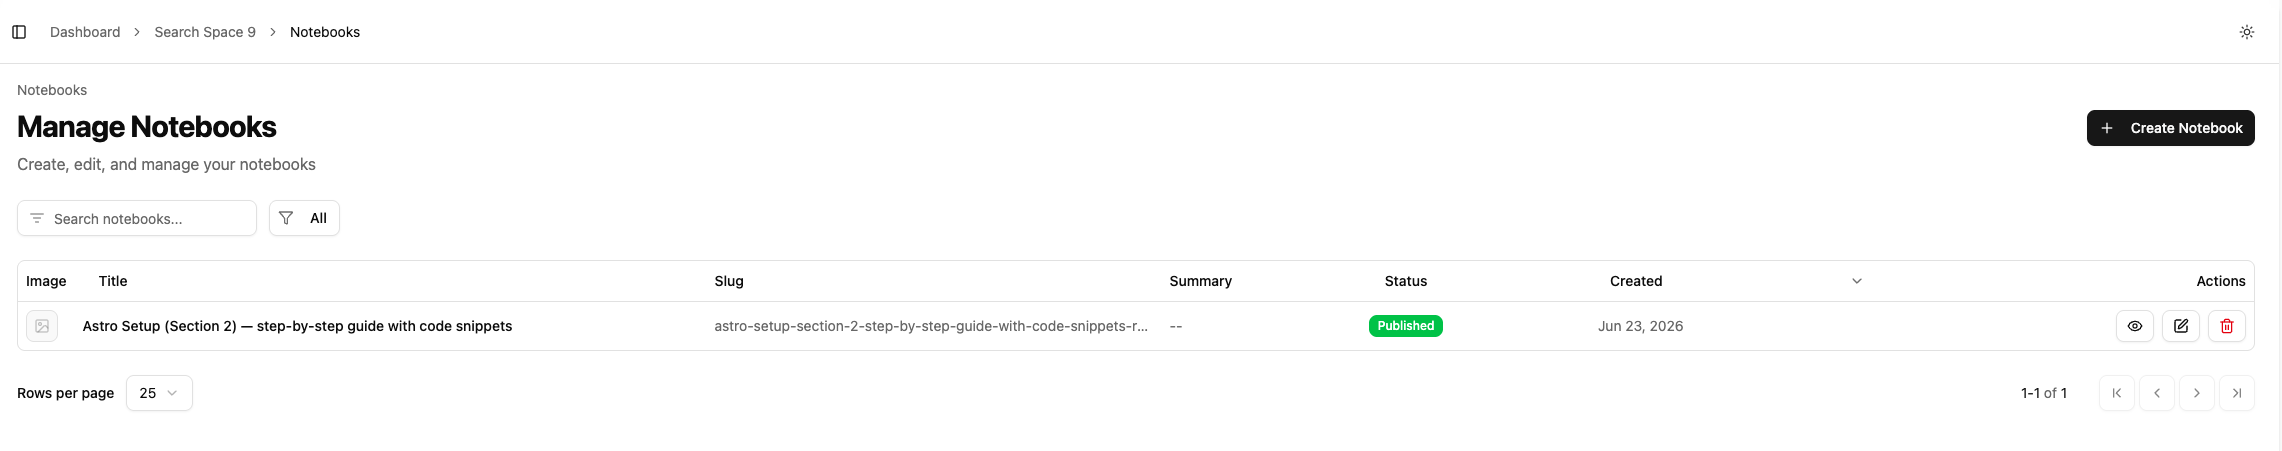
\includegraphics[width=0.95\textwidth,height=0.72\textheight,keepaspectratio]{assets/ui/popis_biljeznjica.png}
    \caption{Upravljanje bilježnicama i statusima objave}
    \label{fig:popis-biljeznica}
\end{figure}

Uređivač na slici~\ref{fig:urednik-biljeznice} prikazuje naslov, strukturirane tekstualne blokove, slikovni sadržaj te radnje spremanja i objave. Veza između uređivanja i objave pokazuje da se isti zapis može koristiti kao privatni izvor znanja i kao javna objava.

\begin{figure}[H]
    \centering
    
\includegraphics[width=0.95\textwidth,height=0.72\textheight,keepaspectratio]{assets/ui/uredivanje_biljeznjice.png}
    \caption{Uređivanje strukturiranog sadržaja i objava bilježnice}
    \label{fig:urednik-biljeznice}
\end{figure}

Prostor znanja može koristiti više osoba, ali svaka osoba ne smije imati iste ovlasti. Suradnja se zato uređuje na razini prostora. Vlasnik poziva korisnika adresom elektroničke pošte i dodjeljuje mu ulogu. Urednik mijenja zajednički sadržaj i poveznike, dok pregledavatelj pristupa dokumentima, bilježnicama i razgovoru bez radnji za izmjenu zajedničkih izvora. Član može napustiti prostor, a vlasnik promijeniti njegovu ulogu ili ga ukloniti. Prilagodba navigacije olakšava korištenje, ali poslužiteljska provjera ostaje mjerodavna za svaku zaštićenu operaciju.

Obrazac za pozivanje i popis članova prikazani su na slici~\ref{fig:clanovi-prostora}. Prikazane uloge i radnje potvrđuju da se suradnja ne temelji samo na dijeljenju poveznice, nego na trajnom članstvu s određenim ovlastima.

\begin{figure}[H]
    \centering
    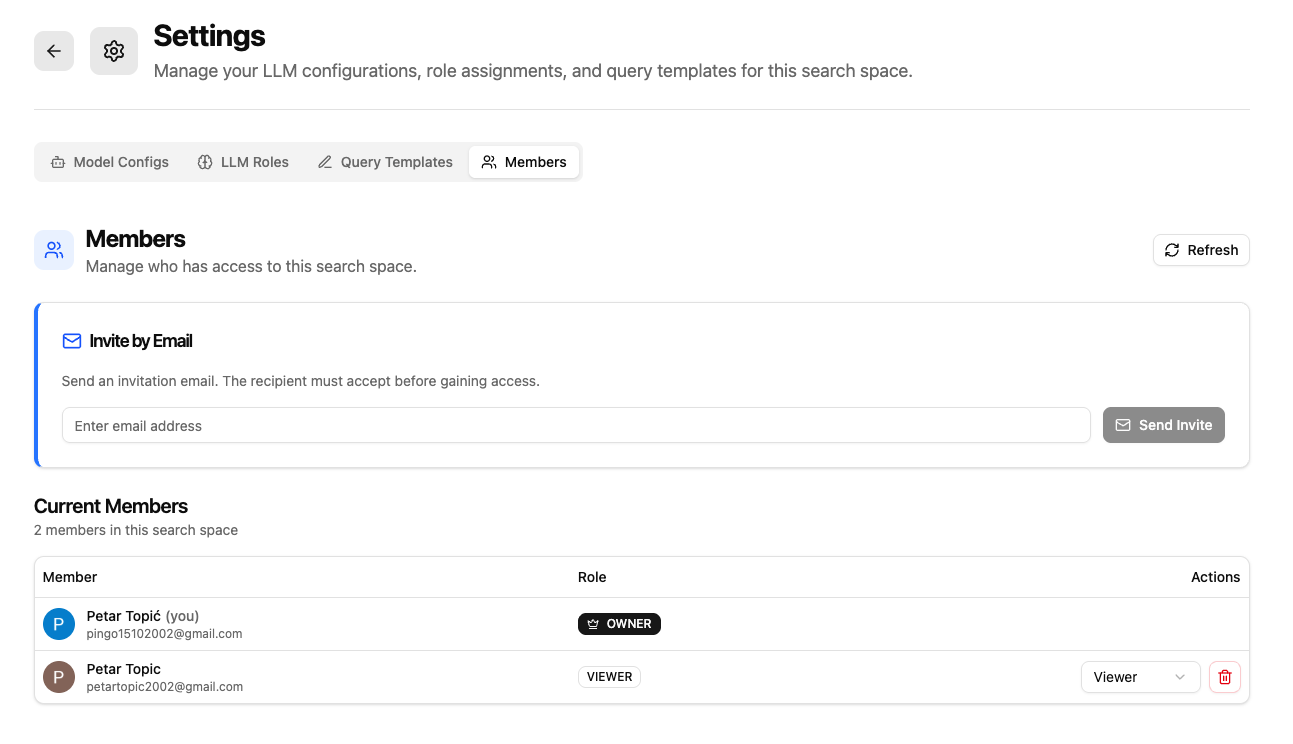
\includegraphics[width=0.95\textwidth,height=0.72\textheight,keepaspectratio]{assets/ui/clanovi_prostora.png}
    \caption{Upravljanje članovima i ulogama unutar prostora znanja}
    \label{fig:clanovi-prostora}
\end{figure}

Razgovorni dio sustava ovisi o odabranom jezičnom modelu i vjerodajnici pružatelja. Konfiguracija modela zato odvaja ključ API od načina uporabe modela u prostoru znanja. Korisnik pohranjuje ključ, a zatim stvara imenovane konfiguracije koje se mogu pregledavati, mijenjati i uklanjati. Isti spremljeni ključ može se povezati s više konfiguracija bez ponovnog unosa. Za brze zadatke, strateško zaključivanje i dugi kontekst mogu se odabrati različiti modeli, dok aktivna konfiguracija određuje i jezik odgovora. Ključ se ne čuva u otvorenom obliku, a sučelje nakon spremanja prikazuje samo njegov skraćeni oblik.

Konfiguracije i njihove uloge prikazane su na slici~\ref{fig:konfiguracije-modela}. Naziv, pružatelj i odabrani model objašnjavaju gdje se konfiguracija primjenjuje, dok skraćeni prikaz ključa potvrđuje da se tajni podatak ne vraća korisničkom sučelju u cijelosti.

\begin{figure}[H]
    \centering
    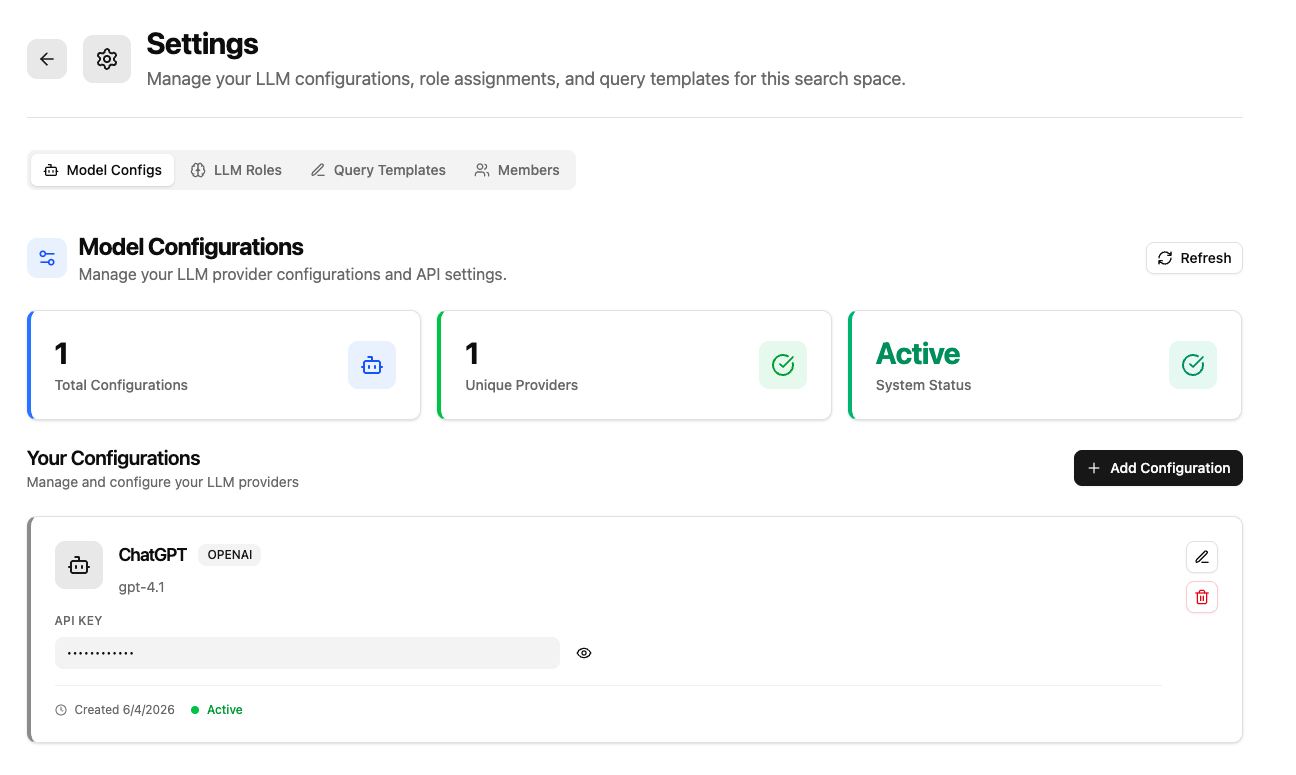
\includegraphics[width=0.95\textwidth,height=0.72\textheight,keepaspectratio]{assets/ui/konfiguracija_modela.png}
    \caption{Konfiguracije jezičnih modela i njihove uloge u prostoru znanja}
    \label{fig:konfiguracije-modela}
\end{figure}

Pozivi jezičnih modela stvaraju trošak, pa sustav taj dio prikazuje kroz kredite. U pregledu pretplate dostupni su trenutačni paket, mjesečno ograničenje te iskorišteni i preostali krediti. Prije pokretanja operacije koja se naplaćuje poslužitelj provjerava raspoloživo stanje. Ako korisnik nema dovoljno kredita, zahtjev se prekida prije poziva modela, čime se sprječava nastanak troška koji nije moguće evidentirati unutar njegova paketa.

Konačni se trošak agentskog odgovora određuje nakon završetka prijenosa odgovora. Povratni poziv biblioteke LangChain zbraja ulazne i izlazne tokene svih poziva modela unutar jednoga agentskog ciklusa, uključujući njegove međukorake. Podaci o broju tokena i korištenom modelu zatim se predaju redu za pozadinsku obradu. Pozadinski proces prema cjeniku modela izračunava broj kredita te u jednoj transakciji povećava potrošnju pretplate i stvara zapis \texttt{UsageRecord}. Budući da zapis sadrži vrstu operacije, prostor znanja, model, broj tokena i broj kredita, potrošnja se može analizirati po korisniku i namjeni.

Administratorski računi, označeni svojstvom \texttt{isSuperuser}, izuzeti su od kreditnih ograničenja. Izuzeće se provjerava prije pokretanja operacije i ponovno tijekom obrade zadatka za oduzimanje kredita. Time se izbjegava naplata čak i ako su administratorska prava dodijeljena nakon predavanja zadatka. Krediti se ne oduzimaju ni kada je poziv modela izveden ključem platforme umjesto korisnikovim spremljenim ključem API. Dodatak~\ref{app:pracenje-potrosnje} prikazuje prikupljanje podataka o tokenima, predavanje obračuna u red, provjeru izuzeća i transakcijsko spremanje potrošnje.

Plaćeni se paketi ugovaraju putem usluge Stripe. Iz pregleda pretplate korisnik pokreće postupak naplate ili otvara korisnički portal u kojem može upravljati postojećom pretplatom, uključujući njezino otkazivanje i ponovno aktiviranje.

Slika~\ref{fig:korisnicka-pretplata} prikazuje aktivni paket, stanje kredita i radnju za upravljanje pretplatom. Takav objedinjeni prikaz korisniku omogućuje da prije pokretanja zahtjevnije operacije procijeni raspoloživu potrošnju i po potrebi promijeni paket.

\begin{figure}[H]
    \centering
    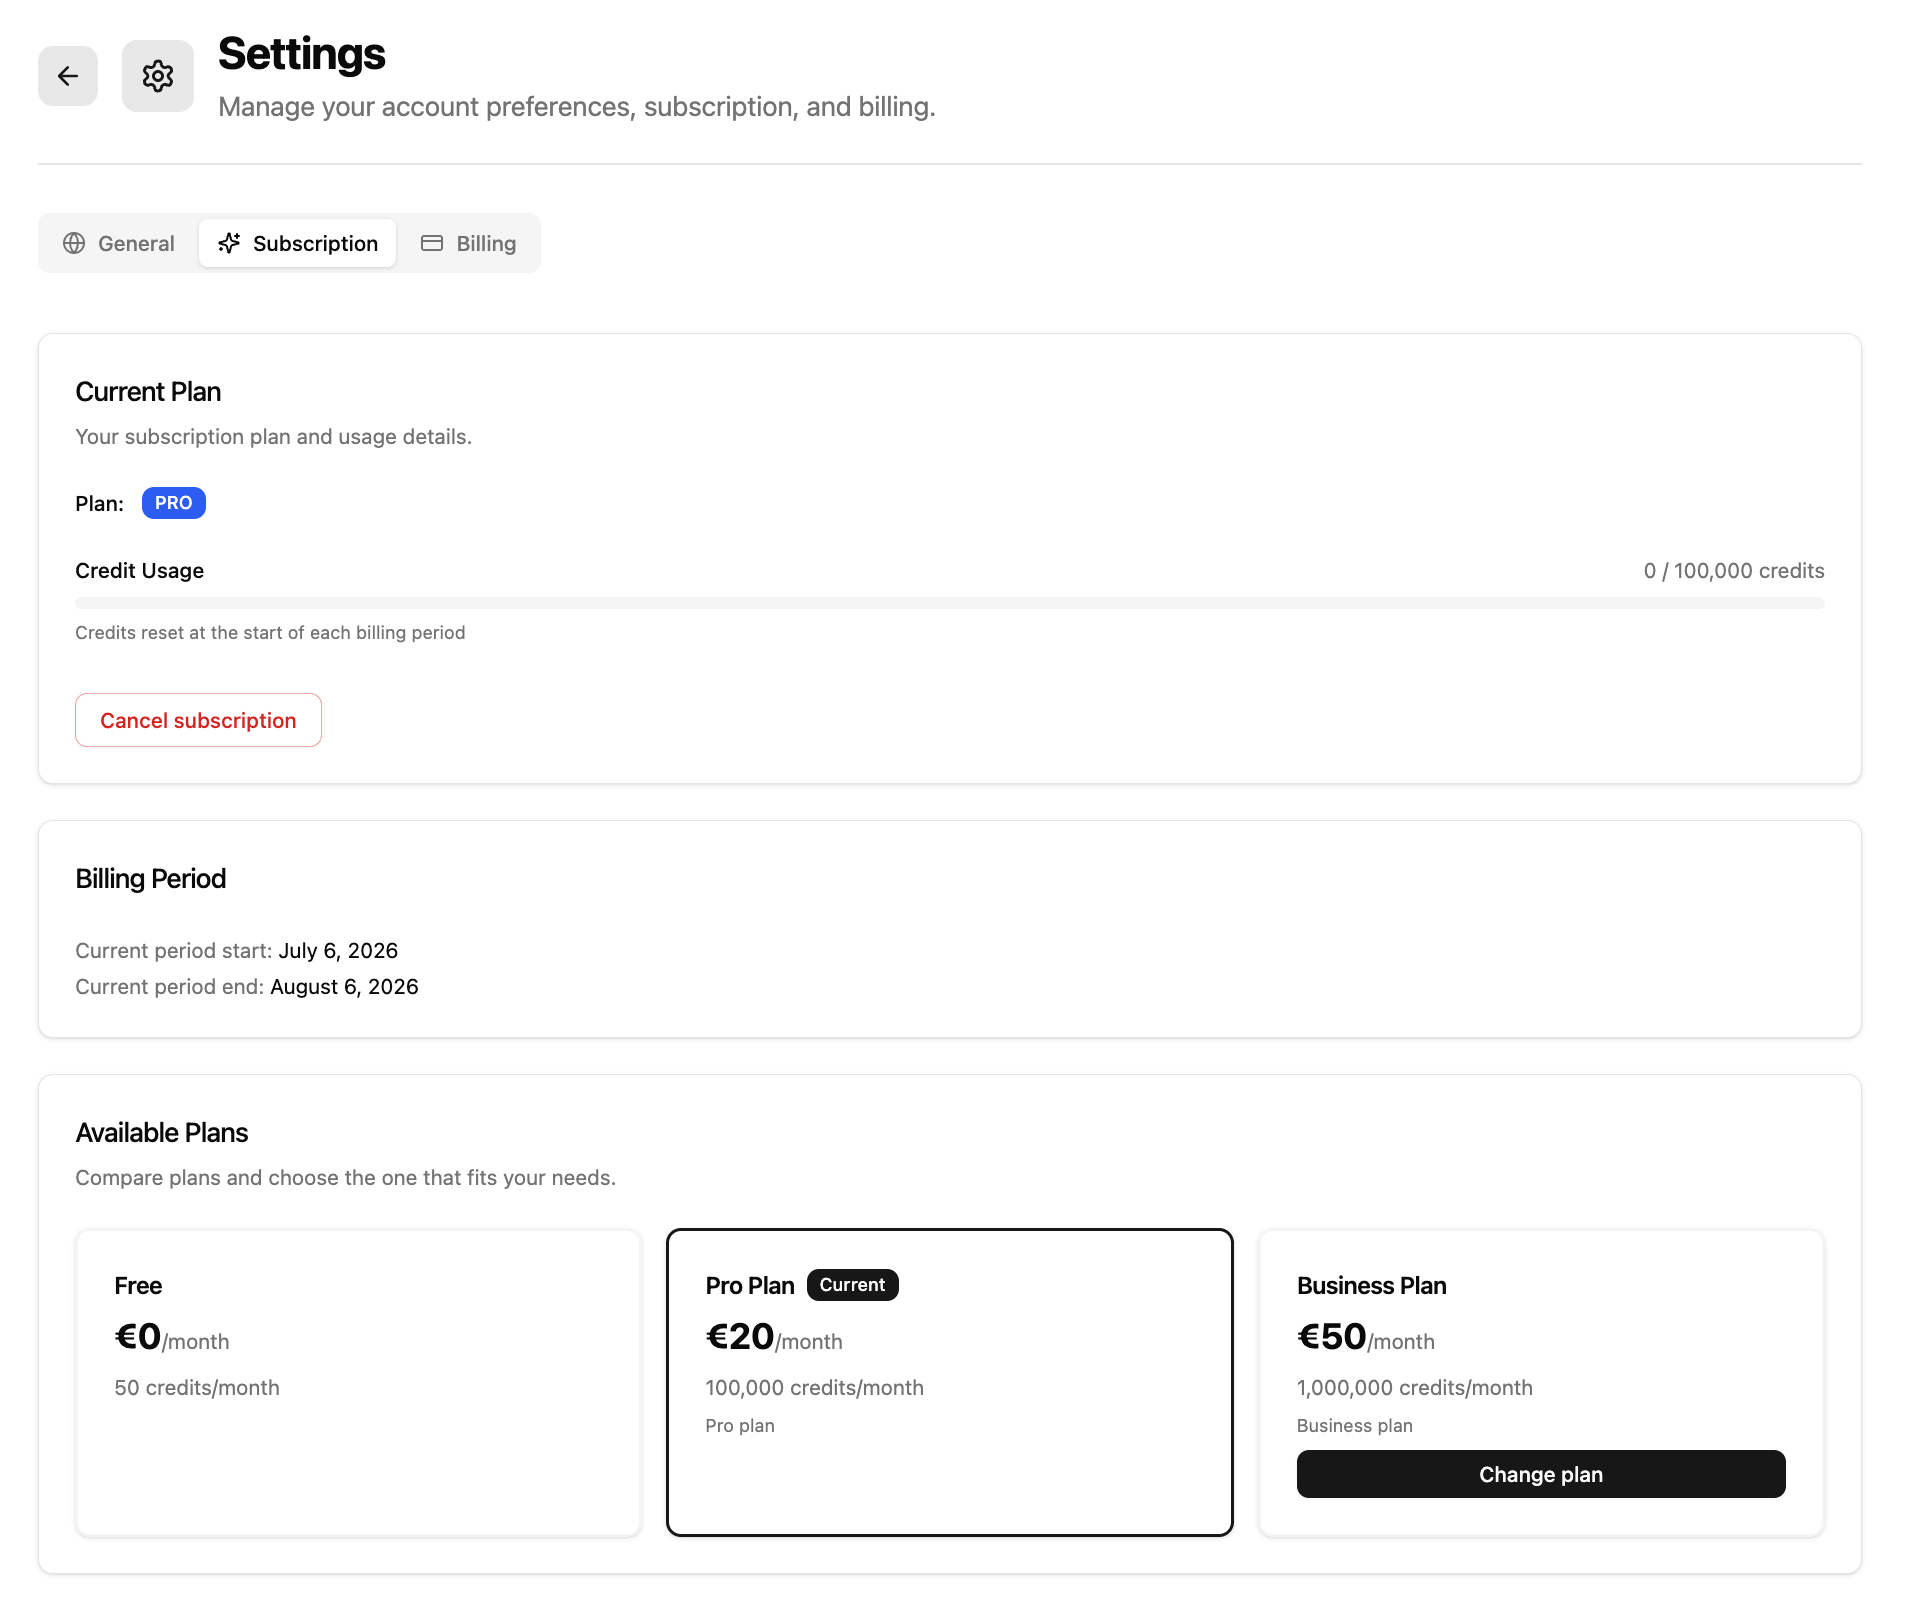
\includegraphics[width=0.9\textwidth,height=0.72\textheight,keepaspectratio]{assets/ui/prikaz_korisnikove_pretplate.png}
    \caption{Pregled korisničke pretplate i potrošnje kredita}
    \label{fig:korisnicka-pretplata}
\end{figure}

Dodatak~\ref{app:stripe-integracija} prikazuje programski kôd za stvaranje Stripeove sesije naplate i obradu povratnih događaja. Provjera potpisa potvrđuje da je događaj poslao Stripe, dok pohrana identifikatora događaja sprječava da ponovljena dostava isti događaj primijeni više puta.

\subsection{Aplikacija namijenjena administratorima sustava}

Administratorsko sučelje odvojeno je od rada u prostoru znanja jer njegove radnje vrijede za cijelu platformu. U pregledu korisnika administrator može pretraživati račune, stvoriti novog korisnika, promijeniti osnovne podatke, dodijeliti ili ukloniti administratorska prava te aktivirati ili deaktivirati račun. Brisanje je izdvojena radnja jer zajedno s računom uklanja i podatke povezane pravilima baze.

Na slici~\ref{fig:administracija-korisnika} prikazani su pretraživanje, stanje računa, korisnička uloga i dostupne administratorske radnje. Njihov zajednički prikaz omogućuje razlikovanje svakodnevnog uređivanja računa od radnji koje mijenjaju pristup cijelom sustavu.

\begin{figure}[H]
    \centering
    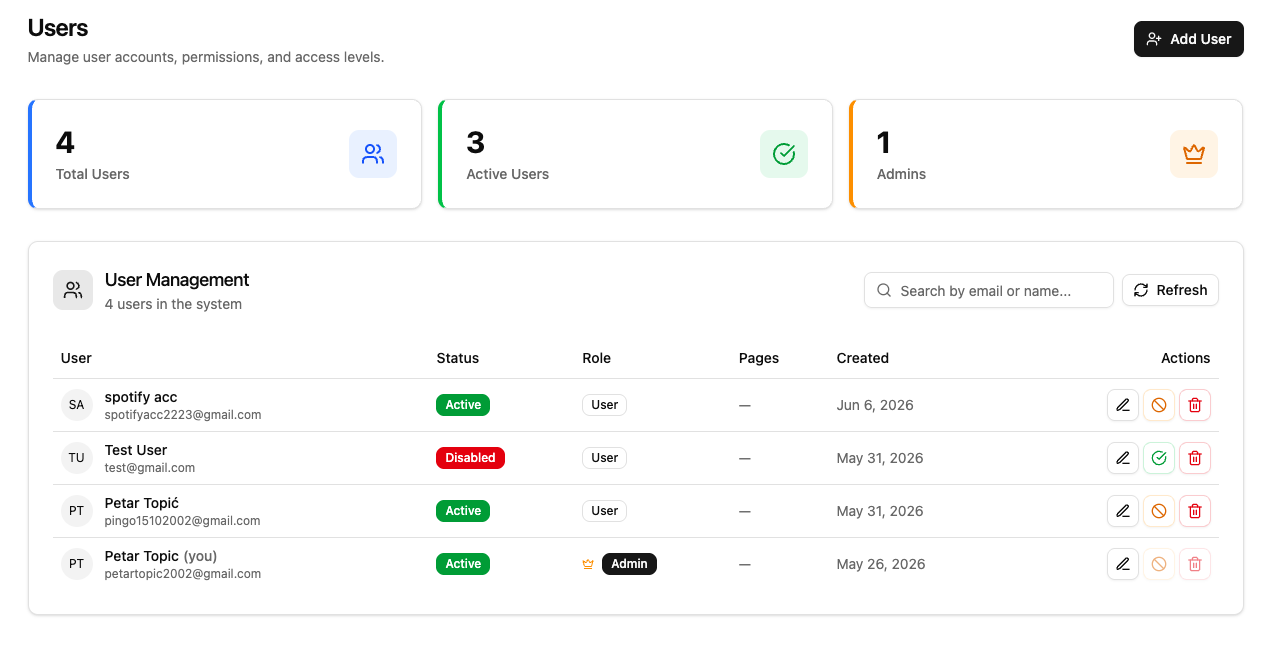
\includegraphics[width=0.95\textwidth,height=0.72\textheight,keepaspectratio]{assets/ui/administrator_upravljanje_korisnicima.png}
    \caption{Administratorsko upravljanje korisničkim računima}
    \label{fig:administracija-korisnika}
\end{figure}

Administratoru je potreban i sažetak stanja cijele instalacije. Stranica sustava prikazuje broj korisnika, aktivnih korisnika, administratora, prostora znanja, dokumenata i razgovora. Operativni dio pregleda obuhvaća broj trenutačno aktivnih radnji te ukupan broj uspješno i neuspješno završenih radnji. Uz zbirne vrijednosti prikazuje se potrošnja po korisniku, s mogućnošću pretraživanja i osvježavanja podataka. Ti podaci služe praćenju platforme, dok detaljni dnevnici pojedinog prostora ostaju dostupni njegovim članovima prema ovlastima.

Slika~\ref{fig:administratorski-pregled} objedinjuje zbirne pokazatelje sustava i tablicu potrošnje po korisniku. Zbirne vrijednosti daju opći pregled aktivnosti platforme, dok pojedinačni zapisi omogućuju provjeru raspodjele potrošnje bez ulaska u svaki korisnički račun.

\begin{figure}[H]
    \centering
    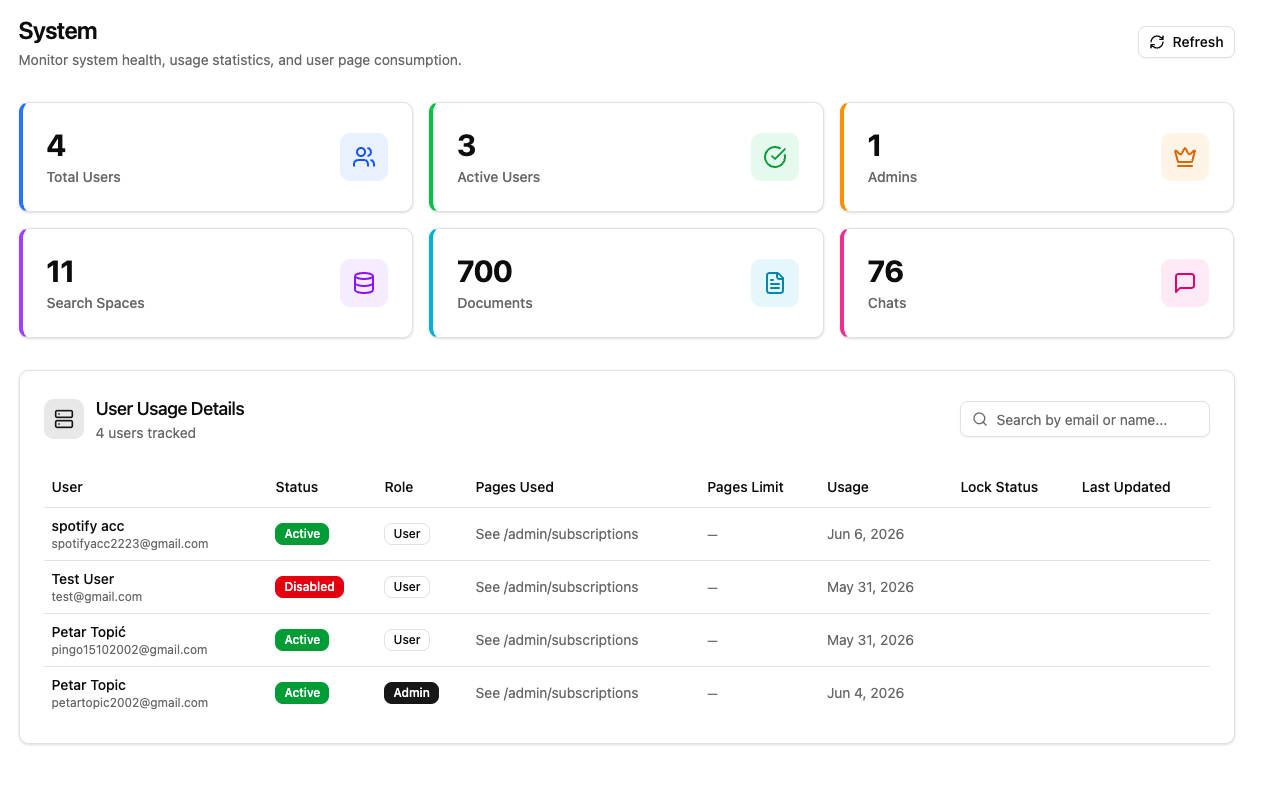
\includegraphics[width=0.95\textwidth,height=0.72\textheight,keepaspectratio]{assets/ui/administrator_pregled_stanja_sustava.png}
    \caption{Administratorski pregled pokazatelja sustava i potrošnje korisnika}
    \label{fig:administratorski-pregled}
\end{figure}

Upravljanje pretplatama povezuje pravila paketa s potrošnjom korisnika. Administratorski pregled obuhvaća besplatne i plaćene pakete, potrošnju svih korisnika, promjenu paketa pojedine pretplate te ponovno postavljanje iskorištenih kredita. Ograničenja, primjerice dopušteni broj obrađenih stranica ili mjesečna potrošnja, mijenjaju se kroz definiciju plana. Poslužiteljska usluga nakon promjene primjenjuje novo ograničenje na pretplate tog plana, čime se pravilo održava u bazi umjesto u korisničkom sučelju. Podaci o kupnji i stanju plaćene pretplate usklađuju se sa Stripeom, dok administratorsko sučelje omogućuje nadzor paketa i korištenja unutar aplikacije. Administratorske rute dodatno provjeravaju oznaku \texttt{isSuperuser}, pa članstvo ili vlasništvo nad prostorom samo po sebi ne daje pristup ovim funkcionalnostima.

Na slici~\ref{fig:administracija-pretplata} prikazane su definicije paketa, pripadajuća ograničenja i korisničke pretplate. Administrator tako na jednom mjestu može povezati pravila pojedinog paketa sa stvarnim stanjem njegove uporabe.

\begin{figure}[H]
    \centering
    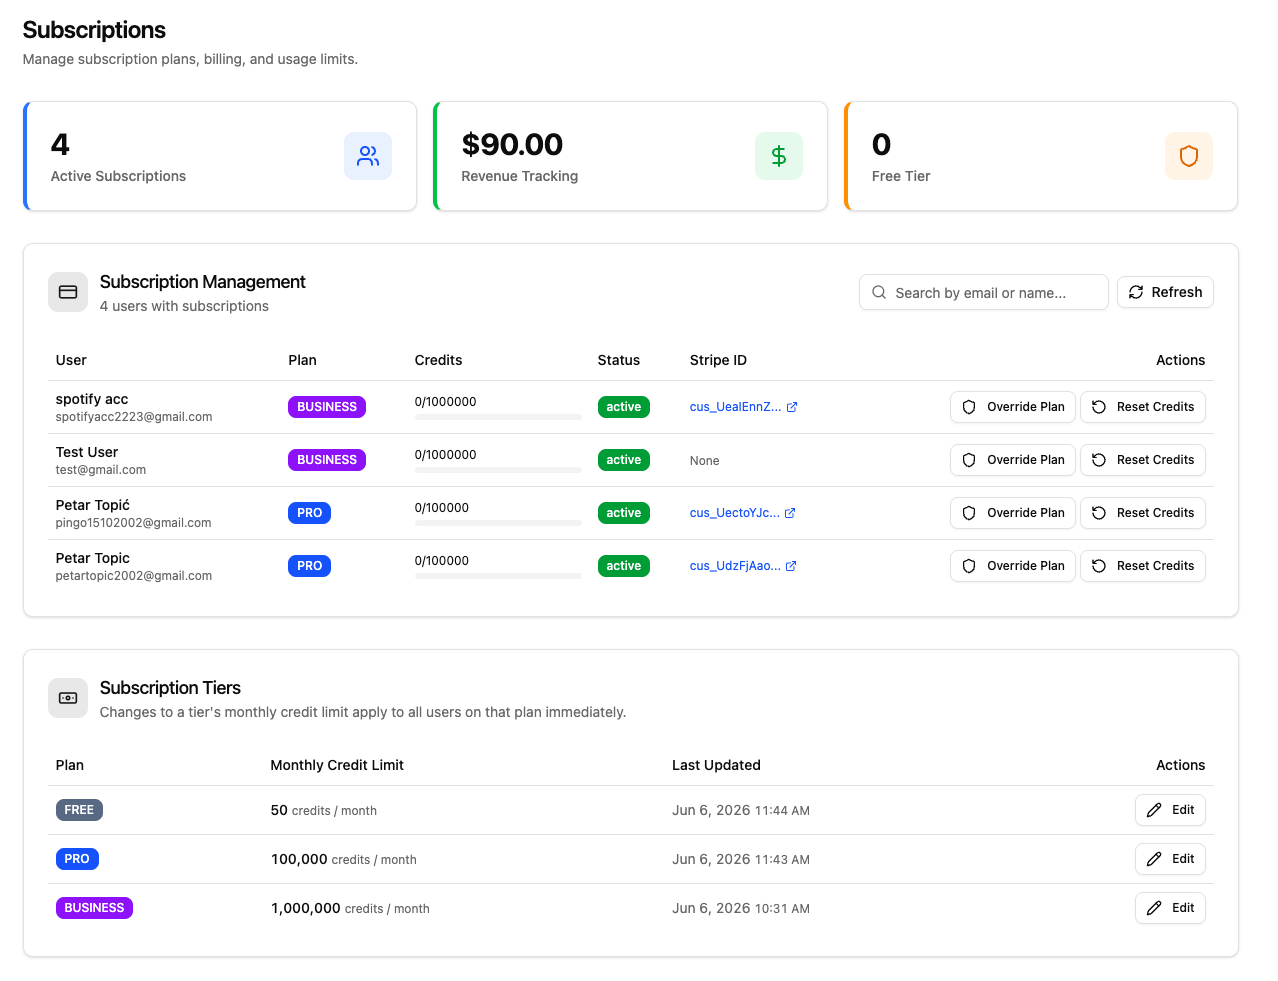
\includegraphics[width=0.95\textwidth,height=0.72\textheight,keepaspectratio]{assets/ui/administrator_upravljanje_pretplatama.png}
    \caption{Administratorsko upravljanje paketima i pretplatama}
    \label{fig:administracija-pretplata}
\end{figure}

Podjela na neregistrirane korisnike, registrirane članove prostora i administratore odražava tri razine odgovornosti. Javni korisnik može pregledati samo namjerno objavljen sadržaj, član radi unutar ovlasti pojedinog prostora, a administrator upravlja računima, paketima i stanjem sustava. Tako se funkcionalnosti upravljanja znanjem odvajaju od poslova upravljanja cijelom platformom.

% ----------------------------------------------------------------
% Chapter 4: Zaključak
% ----------------------------------------------------------------
\chapter{Zaključak}

Polazište rada bio je problem raspršenih izvora znanja. Dokumenti, mrežne stranice, videozapisi i vanjske usluge korisniku su korisni samo ako ih može pronaći, povezati i provjeriti u trenutku kada postavlja pitanje. Cilj rada bio je razviti mrežnu platformu koja takve izvore organizira u prostore znanja i omogućuje razgovorno pretraživanje uz pomoć postojećih velikih jezičnih modela. Poseban je naglasak stavljen na dohvat sadržaja povezanog s pitanjem i prikaz citata, kako bi korisnik uz odgovor mogao pregledati i izvorni kontekst.

Razvijeni sustav pokriva cijeli tijek od unosa izvora do odgovora s citatima. Izvori se obrađuju asinkrono, dijele na manje cjeline, pretvaraju u vektorske ugradnje i pripremaju za semantičko i hibridno pretraživanje. Agentski sloj zatim povezuje dohvat s razgovornim sučeljem. Odgovor se prenosi postupno, a citati ga povezuju s pronađenim ulomcima. Uz taj temeljni tijek razvijeni su suradnja unutar prostora znanja, upravljanje ulogama i ovlastima, javna objava bilježnica, dijeljenje razgovora, periodičko indeksiranje vanjskih izvora te praćenje pozadinskih zadataka. Pretplatnički paketi, evidencija potrošnje i integracija sa Stripeom pokrivaju trošak korištenja modela, dok administratorsko sučelje služi nadzoru korisnika, paketa i stanja platforme.

Postavljeni cilj ostvaren je jer korisnik u istom sustavu može stvoriti prostor znanja, dodati ili povezati izvore, pratiti njihovu obradu i nad indeksiranim sadržajem postavljati pitanja prirodnim jezikom. Organizacija podataka po prostorima i poslužiteljske provjere ovlasti omogućuju da isti korisnik surađuje u više odvojenih baza znanja s različitim ulogama. Platforma se zato može primijeniti za pretraživanje projektne i interne dokumentacije, pripremu sažetaka i analiza te dijeljenje uređenog znanja unutar tima. Vrijednost rješenja nije u razvoju novog jezičnog modela, nego u povezivanju postojećih modela s privatnim i promjenjivim izvorima te u očuvanju veze između odgovora i korištenog sadržaja.

Ograničenja sustava proizlaze iz ovisnosti o dostupnosti vanjskih modela i povezanih usluga te iz kvalitete sadržaja koji korisnik unese. Pronađeni izvori i prikazani citati olakšavaju provjeru, ali sami po sebi ne jamče da je generirani odgovor potpun ili da je sadržaj pravilno protumačen. Rad također nije obuhvatio uvježbavanje vlastitog modela ni sustavnu usporedbu različitih modela i konfiguracija dohvata. Daljnji razvoj može uključiti izradu skupa reprezentativnih pitanja i očekivanih izvora za ponovljivu procjenu kvalitete dohvata i odgovora. Drugi je smjer unapređenje nadzora vanjskih poveznika kroz detaljnije pokazatelje sinkronizacije, automatsko prepoznavanje zastarjelog sadržaja i jasnije postupke oporavka nakon neuspjele obrade.
